% nie rusza�
\RequirePackage{ifpdf}
\newif\ifelektroniczna
\newif\ifjednostronna
\newif\ifprojektInzynierski

%%%%%%%%%%%%%%%%%%%%%%%%%%%%%%%%%%%%%%%%%%%%%%%%%%%%%%%%%%%%%%%%%%%%%%%%%%%%
% USTAWIENIA GLOBALNE I domy�lna �cie�ka do plik�w z obrazkami, kodowanie itp. 
% okre�lone s� w drugiej sekcji ustawie�

% czy projekt czy praca magisterska
%\projektInzynierskitrue % projekt
\projektInzynierskifalse % praca magisterska

% czy wersja elektroniczna (pdf z kolorowymi linkami) czy nie (np. do druku)
\elektronicznatrue
%\elektronicznafalse

% czy jednostronna (recenzent), czy dwustronna (do akt);
% UWAGA: to nie jest dyrektywa dla drukarki; nie zmienia sposobu wydruku, 
% tylko to, w jaki spos�b rozpoczynane s� rozdzia�y, ustawiane marginesy
% itp.

\jednostronnafalse
%\jednostronnatrue

%%%%%%%%%%%%%%%%%%%%%%%%%%%%%%%%%%%%%%%%%%%%%%%%%%%%%%%%%%%%%%%%%%%%%%%%%%%%


% nie rusza�
\ifjednostronna
    \def\strony{oneside,openany}
\else
    \def\strony{twoside,openright}
\fi

\ifpdf
    % uwaga, ustawiaj�c co� innego ni� 12 sprawd� uk�ad strony tytu�owej (marginesy)
    \documentclass[pdftex,12pt,a4paper,\strony,colorlinks,nocenter,noupper,crosshair]{thesis}
    \usepackage[pdftex]{graphicx}
    \pdfcompresslevel=1
\else    
    \documentclass[12pt,a4paper,\strony,nocenter,noupper,crosshair]{thesis}
    \usepackage{graphicx}
\fi

% nie rusza�
\usepackage{url}
\usepackage{stronatytulowa}

%%%%%%%%%%%%%%%%%%%%%%%%%%%%%%%%%%%%%%%%%%%%%%%%%%%%%%%%%%%%%%%%%%%%%%%%%%%%
% USTAWIENIA GLOBALNE - cz�� 2
%

% kodowanie dokumentu
%\usepackage[utf8]{inputenc}   % linuks/windows/mac; pozwala na �atwe mieszanie znak�w z r�nych j�zyk�w
\usepackage[cp1250]{inputenc} % windows

% dane 
\ifprojektInzynierski
    \def\rodzaj{Projekt in�ynierski}
\else
    \def\rodzaj{Praca dyplomowa magisterska}
\fi
%\def\rodzaj{Praca przej�ciowa}

% stan na 2011-2012
\ifprojektInzynierski
    \def\wydzial{Automatyki Elektroniki i~Informatyki}
\else
    \def\wydzial{In�ynierii Biomedycznej}
\fi

\def\tytul{TYTUL \\PRACY} % Prosz� u�y� i ma�ych, i du�ych liter!
\def\autor{Autor: AUTOR PRACY} %Jan Kowalski a NIE JAN KOWALSKI

% tytu� i autor dla pdfa - najcz�ciej jw, ale bez podzia�u na liniie i BEZ POLSKICH LITER
\def\tytulpdf{TYTUL DLA PDFa}
\def\autorpdf{AUTOR DLA PDFa}

% promotor
\def\promotor{Kieruj�cy prac�: PROMOTOR} % prof. nzw. dr hab. in�. dr n.med doc. Jan Kowalski

% z konsultantem/bez konsultanta
%\def\konsultant{Konsultant: Konsultant} prof. nzw. dr hab. in�. dr n.med doc. Jan Nowak
\def\konsultant{}

\def\data{Gliwice, MIESI�C, ROK} % uwaga na wielko�� liter: grudzie� 2012/czerwiec 2012/..

% do pdfa
\def\slowakluczowe{SLOWA,KLUCZOWE}

% �cie�ka do obrazk�w
\graphicspath{{./rysunki/}}

% ustawienia dla pdfa
\ifpdf
\ifelektroniczna
     \usepackage[pdfusetitle=true,
	  pdfsubject={\tytulpdf},
	        pdfkeywords={\slowakluczowe}, 
		pdfcreator={\autorpdf},
		pdfstartview=FitV,
		linkcolor=blue,
		citecolor=red,
		]{hyperref}
\fi                 
\fi


\usepackage{layout}% poka� marginesy

% Nazwa za��cznik�w 
\def\appendixname{Za��cznik}
%%%%%%%%%%%%%%%%%%%%%%%%%%%%%%%%%%%%%%%%%%%%%%%%%%%%%%%%%%%%%%%%%%%%%%%%%%%%

% nie rusza� (cho� chwilowo niepotrzebne)
%	\author{\autor}
%	\title{\tytul}
%	\date{\data}
%

% === PAKIETY ===

% �adne czcionki dla PDF + ustawienia spolszczaj�ce
\usepackage{t1enc,amsmath}
\usepackage[OT4,plmath]{polski}

% potrzebne dla strony tytu�owej:
\usepackage{helvet} 

% pierwszy paragraf w rozdziale/sekcji powinien by� wci�ty
\usepackage{indentfirst}

% marginesy
%\usepackage{anysize}
%\marginsize{3cm}{2.5cm}{2.5cm}{2.5cm}%LPGD
%\setlength{\textheight}{24cm}
% za spraw� thesis
%\textwidth 150mm
%\textheight 225mm

% czcionki matematyczne
\usepackage{amsfonts}

% rysunki z�o�one z wielu [pod]rysunk�w
\usepackage{subfig}
\captionsetup[subfigure]{justification=centerfirst}

% mo�liwo�� sklejania wierszy tabeli
\usepackage{multirow}

% mo�liwo�� wklejania adres�w - jest ju� w��czony wy�ej
%\usepackage{url}

% ulepszona obs�uga cytowa�
\usepackage{cite}

% listingi
\usepackage{listings}
% domy�lne ustawienia (niestety utf8 nie jest akceptowany)
%\lstset{language={Matlab},inputencoding=cp1250}}
%\lstset{language={Matlab},inputencoding=latin2}}
\lstset{language={Java},inputencoding=latin2} % powinno pasowa� te� do C#

% \addcontentsline nie dzia�a za dobrze w po��czeniu z hyperref, ale to nie dzia�a z klas� thesis
%\usepackage[nottoc]{tocbibind}

% strona po cleardoublepage powinna by� pusta, nie z nag��wkami
\usepackage{cleardpempty}

% == opcjonalne

% wymu� po�o�enie grafiki (itp.) przez [H]
\usepackage{float} 

% znak promila i inne znaki specjalne
%\usepackage{textcomp}

% je�li trzeba obr�ci� stron� (wstawi� co� w orientacji poziomej), u�yj tych pakiet�w
%\ifpdf\usepackage{pdflscape}\else\usepackage{lscape}\fi

% je�li potrzebujesz d�ugich tabeli (wiele stron)
%\usepackage{longtable}

% === POLECENIA DODATKOWE ===

% wektor w tek�cie
\def\vec#1{\ensuremath{\mathbf{#1}}}

% anglicyzmy i �acinizmy
\def\ang#1{ang.~\emph{#1}}
\def\lat#1{�ac.~\emph{#1}}

% proste e (jako podstawa logarytmu naturalnego) we wzorach i w tek�cie:
\def\e{\ensuremath{\textrm{\normalfont{}e}}}

% znak stopnia [jak w "5 stopni"]
\def\stopien{\ensuremath{^{\circ}}\protect\space}

% notatki na marginesie
\def\fixme#1{\marginpar{\tiny{}#1}}
%\def\fixme#1{} % gdy nie chcemy ich drukowa�, wystarczy zast�pi� powy�sze tym

%ODNOSNIKI 
% �eby wykorzysta� przypis dwukrotnie; druga wersja gorzej dzia�a�a w po��czeniu 
% z hyperref; czyli \footnote{blablabla \label{przypisX}} + \footnotereuse{przypisX}
%\newcommand{\footnreuse}[1]{\raisebox{1ex}{\scriptsize{}\protect\ref{#1}}}

% == �RODOWISKA DLA TWIERDZE�, LEMAT�W itp. ===
\newtheorem{twierdzenie}{Twierdzenie}[chapter]
\newtheorem{wlasnosc}{W�asno��}[chapter]
\newtheorem{lemat}{Lemat}[chapter]
\newenvironment{dowod}{\parindent=0pt{\bf Dow�d. }}{\begin{flushright}$\square$\end{flushright}}

% === RACZEJ NIE RUSZA� ===

%\usepackage{makeidx}
%\makeindex
%\usepackage{threeparttable}
%\usepackage[small,center]{caption2}

\def\captionlabeldelim{.}

%\usepackage{geometry}
%GATHER{thesis.bib}
%\usepackage[twoside]{geometry}
%\geometry{ lmargin=3.5cm, rmargin=2.5cm, tmargin=3cm, bmargin=3cm,
%headheight=1cm, headsep=0.5cm, footskip=0pt }

\linespread{1}
\chapterfont{\Huge\bfseries}
\sectionfont{\bfseries\Large}
\subsectionfont{\bfseries\large}
\institutionfont{\bfseries}%\mdseries}
\def\captionlabelfont{\bfseries}

\renewcommand{\figureshortname}{Rys.}
\renewcommand{\tableshortname}{Tab.}

\renewcommand\floatpagefraction{.9}
\renewcommand\topfraction{.9}
\renewcommand\bottomfraction{.9}
\renewcommand\textfraction{.1}
\setcounter{totalnumber}{50}
\setcounter{topnumber}{50}
\setcounter{bottomnumber}{50}

\newcommand{\topcaption}{%                  % robi podpis nad tabelk� z odst�pem po podpisie
   \setlength{\abovecaptionskip}{0pt}%
   \setlength{\belowcaptionskip}{10pt}%
   \caption}


\usepackage{color}
% marginesy
\usepackage{anysize}
\marginsize{3cm}{2.5cm}{2.5cm}{2.5cm}%LPGD
%\setlength{\textheight}{24cm}
% za spraw� thesis
%\textwidth 150mm
%\textheight 225mm

\begin{document}
%
\bibliographystyle{acm}
%

%
%\stronatytulowa
\titlepage
%\ \cleardoublepage % je�li dwustronnie, to druga strona powinna by� pusta
\frontmatter 
%\maketitle

%\tocbibname

\tableofcontents \listoffigures \listoftables
%\listofacros
%\input{abbrev_body}
%\newpage
%\input{spis_oznaczen}

\mainmatter % <--- to + frontmatter powy�ej odpowiada za fakt, �e numerowanie jest od 1!
\chapter{Wprowadzenie}
% \setlength{\parindent}{50pt} tak si� robi wci�cia
\section{Streszczenie}
W~pracy przedstawiono model opisuj�cy odpowied� uk�adu immunologicznego na~rozwijaj�cy si� w~organizmie nowotw�r. Model ten oparty jest na~modelu de Pillis'a oraz~modelu Isaeva i~Osipov'a \cite{1}. Obejmuje on rozw�j kom�rek nowotworowych w~organizmie oraz~odpowied� uk�adu immunologicznego -- w~tym limfocyt�w naciekaj�cych nowotw�r TIL (ang. Tumor Infiltrating Lymphocytes), tak zwanych ,,naturalnych zab�jc�w'', czyli kom�rek NK (ang. Natural Killer cells) oraz limfocyt�w $T_{CD8+}$.
Nast�pnie model zosta� poddany modyfikacji polegaj�cej na~ uwzgl�dnieniu procesu leczenia nowotworu skojarzonymi metodami chemioterapii i~immunoterapii z~u�yciem cytokin: interleukin-2 (IL-2) i~interferon�w alfa (IFN-$\alpha$).

\section{Cel pracy}
Celem pracy by�o:
\begin{itemize}
\item utworzenie modelu rozwoju nowotworu w~organizmie z~uwzgl�dnieniem leczenia skojarzonymi metodami chemioterapii i~immunoterapii,
\item przeprowadzenie symulacji leczenia nowotworu metod� chemioterapii, immunoterapii oraz~skojarzonych metod chemioterapii i~immunoterapii,
\item analiza rozwi�za� modelu opisuj�cego leczenie wy��cznie metod� chemioterapii,
\item analiza rozwi�za� modelu opisuj�cego leczenie wy��cznie metod� immunoterapii,
\item analiza rozwi�za� modelu opisuj�cego leczenie zar�wno metod� chemioterapii, jak~i~immunoterapii.
\end{itemize}

\newpage
\section{Uk�ad pracy}
Praca sk�ada si� z~nast�puj�cych cz�ci:
\begin{itemize}
\item wst�pu teoretycznego zawieraj�cego informacje na~temat rodzaj�w nowotwor�w i~sposob�w ich rozwoju oraz~niekt�rych metod ich leczenia, a~tak�e dotycz�cych budowy i~sposobu dzia�ania uk�adu immunologicznego,
\item przedstawienia zaimplementowanego modelu, na kt�rym przeprowadzano symulacje,
\item opisu dokonanych symulacji i~scenariuszy, wed�ug kt�rych zosta�y przeprowadzone,
\item analizy wynik�w symulacji i~wynikaj�cych z~nich wniosk�w,
\item podsumowania.
\end{itemize}

\chapter{Wst�p}
\section{Procesy nowotworowe}
Nowotworem okre�la si� nieprawid�owe kom�rki w~organizmie, kt�rych wzrost odbywa si� w~spos�b niekontrolowany \cite{1, 2}. Czasami, najcz�ciej w~przypadku zmian zapalnych, naprzemiennie z~poj�ciem nowotw�r, stosowane jest okre�lenie guz \cite{24}. W~zdrowym organizmie wyst�puje r�wnowaga pomi�dzy tempem podzia��w kom�rkowych a~utrat� kom�rek. W~przypadku nowotworu ginie mniej kom�rek ni� przybywa \cite{3}. W~efekcie spontanicznej proliferacji kom�rek nowotworowych sk�adaj�ca si� z nich struktura zaczyna niszczy� narz�d, w~kt�rym wyst�pi� proces nowotworowy. Niekt�re z~tych kom�rek mog� oderwa� si� od~pozosta�ych, przedosta� do~naczy� krwiono�nych i~limfatycznych, a~w~konsekwencji dawa� przerzuty do~innych narz�d�w \cite {2}. Powstawanie nowotworu wi��e si� z~wieloma zmianami materia�u genetycznego. Rozpocz�cie tego procesu zale�y zar�wno od~wagi, jak~i~miejsca, w~kt�rym dana zmiana wyst�pi�a. 
\newline \indent Warto tak�e zwr�ci� uwag� na~zmiany system�w naprawy DNA oraz~zmiany system�w reguluj�cych podstawowe procesy kom�rkowe (na przyk�ad wzrost, r�nicowanie, apoptoz�\footnote{Apoptoza -- �mier� programowana, �mier� samob�jcza kom�rki zachodz�ca w~warunkach fizjologicznych \cite{12}.}). Na~skutek zmian system�w naprawczych dochodzi do~szybkiej i~du�ej niestabilno�ci genomu. Zmiany w~systemach reguluj�cych powoduj� natomiast powolny proces zaburzenia homeostazy kom�rki oraz stopniowo narastaj�c� niestabilno�� genomu. Choroby nowotworowe w~wi�kszo�ci rozwijaj� si� w tym drugim przypadku, dlatego od~pojawienia si� pocz�tkowej zmiany do~klinicznego wykrycia guza mija zazwyczaj wiele lat \cite{3}.

% nowe p1
Transformacja oznacza wielostopniowy proces, podczas kt�rego kom�rki prawid�owe staj� si� z�o�liwe. Ka�dy etap tego procesu odpowiada zmianom genetycznym prowadz�cym do zaburze� wzrostu kom�rek prawid�owych. Dobrze poznany jest rozw�j nowotworu w~przypadku czerniaka sk�ry \cite{24}. \newpage Transformacj� melanocyt�w w~kierunku czerniaka mo�na podzieli�, klinicznie i~histopatologicznie, na pi�� g��wnych etap�w \cite{24}
\begin{itemize}
\item [1.] znami� barwnikowe,
\item [2.] znami� dysplastyczne,
\item [3.] faza radialna wzrostu czerniaka,
\item [4.] faza wertykalna wzrostu czerniaka,
\item [5.] czerniak rozsiany.
\end{itemize}

Zachodz�ce zmiany genetyczne zwi�zane s�~z~r�nymi zmianami fizjologicznymi kom�rki, w~szczeg�lno�ci z \cite{24}
\begin{itemize}
\item samowystarczalno�ci� w~wytwarzaniu sygna��w do wzrostu,
\item niewra�liwo�ci� na inhibitory sygna��w wzrostu,
\item unikaniem programowanej �mierci kom�rek,
\item nieograniczonym potencja�em replikacyjnym, 
\item podtrzymywaniem angiogenezy,
\item inwazj� tkankow�,
\item przerzutami,
\item unikaniem destrukcji immunologicznej.
\end{itemize}  
 
Mechanizmy genetyczne le��ce u~podstaw wy�ej wymienionych zmian fizjologicznych mog� r�ni� si� mi�dzy sob� dla~poszczeg�lnych nowotwor�w. Mimo to, zmiany fizjologiczne~s�~wsp�lne dla~wi�kszo�ci nowotwor�w i~odpowiadaj� zar�wno za prze�ycie, jak i ekspresj� nowotworu \cite{24}.
% nowe k1

\newpage
\section{Budowa uk�adu immunologicznego i~jego znaczenie w~procesie leczenia nowotwor�w}
Na uk�ad immunologiczny sk�adaj� si� mechanizmy odporno�ci swoistej (nabytej) i~nieswoistej (wrodzonej) \cite{4,5,20}. Ich podzia� przedstawiono w~Tab. \ref{r�nice_mi�dzy_nab_a_wrodz}. 
% nowe
Mechanizmy odporno�ci nabytej s�~aktywowane, gdy~mechanizmy odporno�ci wrodzonej nie~zapobiegn� wnikaniu lub~nie~usun� patogenu \cite{20}. 
%nowe

\begin{table}[!htb]
\caption{Mechanizmy obronne odporno�ci nieswoistej i~swoistej \cite{7}.}\label{r�nice_mi�dzy_nab_a_wrodz}
	\centering
	\begin{tabular}{|l|l|l|p{0.47\linewidth}|} \cline{1-2} \cline{4-4} 
		\multicolumn{2}{|c|}{Odporno��} & & Dzia�anie obronne \\ \hline
		\multirow{2}{1cm}{Nieswoista (wrodzona)} & Humoralna & Lizozym & Bakterioliza bakterii Gram dodatnich, liza bakterii Gram-ujemnych po usuni�ciu warstwy liposacharydowej\\ \cline{3-4}
		& & Laktoferyna & Pozbawienie bakterii dost�pu do �elaza poprzez wi�zanie go \\ \cline{3-4}
		& & Transferyna & Pozbawienie bakterii dost�pu do �elaza poprzez wi�zanie go \\ \cline{3-4}
		& & Bia�ka ostrej fazy & Aktywacja limfocyt�w, makrofag�w, dope�niacza na drodze klasycznej \\ \cline{3-4}
		& & Dope�niacz & Uaktywnienie uk�adu dope�niacza\\ \cline{3-4}
		& & Interferony & Hamowanie transformacji limfocyt�w pod wp�ywem mitogen�w \\
		\cline{2-4}
		& Kom�rkowa & Fagocyty & Fagocytoza\\ \cline{3-4}
		& & Eozynofile & Produkcja prostoglandyn PGE1 i PGE2, kt�re hamuj� uwalnianie mediator�w przez kom�rki tuczne i bazofile \\ \cline{3-4}
		& & Kom�rki K & Cytotoksyczno�� zale�na od przeciwcia�\\ \cline{3-4}
		& & Kom�rki NK & Spontaniczne niszczenie kom�rek zaka�onych wirusem\\ \hline \cline{3-4}
		\multirow{2}{3cm}{Swoista (nabyta)} & Humoralna & Immunoglobuliny \\ \cline{3-3}
		& & Limfocyty typu B \\
		\cline{2-3}
		& Kom�rkowa & Limfocyty typu T \\ \cline{1-3}
		\end{tabular}
\end{table}

% nowe
Zasadnicze znaczenie w~odporno�ci organizmu maj� sk�ra, b�ony �luzowe, fagocyty, limfocyty typu T i B\footnote{Limfocyty typu B -- wyspecjalizowane kom�rki uk�adu immunologicznego, kt�rych g��wna funkcja polega na wytwarzaniu przeciwcia�\cite{28}.}, kom�rki NK, przeciwcia�a oraz uk�ad dope�niacza\cite{28}.

Uk�ad dope�niacza wspiera mechanizmy wrodzonej odporno�ci immunologicznej przez~zabijanie drobnoustroj�w za~po�rednictwem lizy, chemotaksj� kom�rek fagocytarnych oraz~u�atwianie procesu fagocytozy. Uk�ad dope�niacza (komplement) tworzy grupa oko�o 40 bia�ek, kt�re zabezpieczaj� organizm przed atakiem drobnoustroj�w. Komplement aktywowany jest kaskadowo (ka�dy kolejny sk�adnik aktywuje nast�pny). \newpage Mo�na wyr�ni� trzy drogi aktywacji dope�niacza\cite{13}:

\begin{itemize}
\item klasyczn�,
\item alternatywn�,
\item lektynow�.
\end{itemize} 

Klasyczna droga aktywacji komplementu zachodzi z~udzia�em swoistych immunoglobulin, kt�re zwi�zane s�~z~powierzchni� drobnoustroj�w. Prowadzi ona~do~�mierci litycznej kom�rki docelowej (bakterioliza).

Znacznie szybsza jest droga alternatywna (properdynowa), poniewa� kszta�tuje si� ona~od~momentu wnikni�cia patogenu. W~tym~przypadku drobnoustroje ulegaj� spontanicznej opsonizacji\footnote{Opsonizacja -- proces u�atwiaj�cy fagocytoz� \cite{13}.} przez~cz�steczki C3b dope�niacza. U�atwia to~ich~poch�anianie przez~kom�rki fagocytarne.

Podczas lektynowej drogi aktywacji nast�puje po��czenie cz�steczki cukru obecnej na powierzchni bakterii z~lektyn� wi���c� mannoz� MBL (ang. Mannose Binding Lectin). Ta~interakcja prowadzi do~rozk�adu czynnik�w C2 i~C4 uk�adu dope�niacza.

Alternatywna droga aktywacji uk�adu dope�niacza jest~podstawowym mechanizmem wrodzonego uk�adu odporno�ciowego. Organizm uruchamia kaskad� nieswoistych reakcji obronnych zanim pojawi� si� swoiste w~stosunku do mikroorganizmu przeciwcia�a. Zapewnia to~oszcz�dno�� czasu, ale alternatywna droga aktywacji oddzia�uje tak�e na~w�asne tkanki, co~ogranicza sprawne funkcjonowanie wielu regulator�w \cite{13}.
% nowe
\newline \newline \indent Funkcjonowanie mechanizm�w nieswoistych jest niezale�ne od~wcze�niejszej styczno�ci organizmu z~czynnikami patogennymi i~pe�ni funkcj� obronn� przed infekcjami i~chorobami b�d�cymi skutkiem dzia�ania czynnik�w �rodowiskowych. Mechanizmy te cechuje mniejsza precyzja, ale s� one zdolne do~szybkiego rozpoznawania i~niszczenia wnikaj�cych drobnoustroj�w. Odporno�� wrodzon� warunkuj� mi�dzy innymi: kom�rki NK, makrofagi, granulocyty, monocyty \cite{4}.

Odporno�� swoista rozpoznaje antygeny\footnote{Antygeny -- zwi�zki wywo�uj�ce reakcje uk�adu immunologicznego; najcz�ciej substancje wielkocz�steczkowe, rozpoznawane swoi�cie poprzez powierzchniowe receptory limfocyt�w \cite{20}.} bardzo precyzyjnie. Jej wa�nymi elementami s� limfocyty typu T, limfocyty typu B, cytokiny oraz przeciwcia�a. Kom�rki te s� zdolne do~wytwarzania nieograniczonej liczby receptor�w. Dodatkowo, je�li dojdzie do~ich kontaktu z~antygenem wytwarza si� pami�� immunologiczna \cite{4}, dzi�ki kt�rej przy~ponownym zetkni�ciu kom�rki danego typu z~odpowiednim antygenem wytwarzana odpowied� immunologiczna jest~szybsza i~silniejsza \cite{20}. W~przypadku limfocyt�w typu T, typ odpowiedzi swoistej okre�lany jest jako kom�rkowy (tj.
zwi�zany z aktywno�ci� kom�rek uk�adu immunologicznego \cite{13}), natomiast dla limfocyt�w typu B -- humoralny (tj. zwi�zany z aktywno�ci� immunoglobulin \cite{13}). \newpage Do mechanizm�w swoistej odporno�ci nale�� \cite{6}:
\begin{itemize}
\item aktywno�� cytokin i~chemokin,
\item cytokinozale�na wrodzona oporno�� leukocyt�w i~innych kom�rek,
\item zabijanie zaka�onych lub~nowotworowych kom�rek przez kom�rki NK, komplement %\footnote{Komplement -- uk�ad dope�niacza, system kaskadowo aktywowanych bia�ek pe�ni�cych znacz�c� rol� w~walce przeciwko czynnikom patogennym, w~utrzymywaniu stanu homeostazy oraz~wzbudzaniu stanu zapalnego\cite{17}.}%
aktywowany lektynami lub~drog� alternatywn�,
\item opsonizacja i~fagocytoza\footnote{Fagocytoza -- usuwanie kompleks�w immunologicznych i~uszkodzonych kom�rek (u�atwienie fagocytozy immunologicznej). Efektywne niszczenie drobnoustroj�w przez fagocyty \cite{13, 14}.}.
\end{itemize}

Pomimo bardzo du�ego znaczenia uk�adu immunologicznego dla organizmu, wiele mechanizm�w jego dzia�ania pozostaje jeszcze niewyja�nionych \cite{4}. \newline \newline Znacz�c� rol� w~oddzia�ywaniu uk�adu immunologicznego na~rozwijaj�cy si� nowotw�r pe�ni�:

\begin{itemize}
\item limfocyty $T_{CD8+}$,
\item kom�rki NK,
\item interferony,
\item interleukiny.
\end{itemize}

W~zwi�zku z~wa�n� funkcj� wy�ej wymienionych kom�rek, uj�to je~w~opisywanym modelu, natomiast ich~znaczenie opisano w~dalszej cz�ci pracy.

% glikoproteiny MHC (Major Histocompatibility Complex)

\subsection{Limfocyty typu T}
Jedn� z~grup limfocyt�w s�~limfocyty typu T, kt�re stanowi� odr�bny rodzaj kom�rek uk�adu immunologicznego. Ich~wyspecjalizowan� funkcj� jest~bezpo�rednie atakowanie obcych antygen�w, na~przyk�ad wirus�w, grzyb�w. Pe�ni� tak�e funkcj� regulatorow� w~obr�bie uk�adu immunologicznego \cite{28}. Limfocyty typu T wytwarzane s� w~szpiku kostnym \cite{7}, a~na~wczesnym etapie �ycia p�odowego trafiaj� do~grasicy (limfocyty grasiczozale�ne), gdzie dojrzewaj�. Nast�pnie opuszczaj� grasic� i~przebywaj� w~r�nych narz�dach uk�adu odporno�ciowego, na przyk�ad �ledzionie, w�z�ach ch�onnych, szpiku kostnym oraz~krwi obwodowej \cite{28}. \newline \newline Limfocyty typu T oznaczane jako CD8+ dziel� si� na~limfocyty \cite{7}:
\begin{itemize}
\item cytotoksyczne $T_{c}$, kt�re odpowiadaj� za~niszczenie kom�rek i~odrzucanie przeszczep�w,
\item supresyjne $T_{s}$, kt�re odpowiadaj� za~hamowanie dzia�ania innych limfocyt�w, reakcji alergicznych i~utrzymanie tolerancji immunologicznej na~w�asne antygeny.
\end{itemize}

Na Rys. \ref{limfocyty_T_cd8+}, na~pomara�czowych, niebieskich i~r�owych polach przedstawiono kolejne podzia�y limfocyt�w typu T wyst�puj�cych w~organizmie. Dodatkowo, na~polach szarych kr�tko opisano funkcj�, jak� one~pe�ni� lub wymieniono ich~charakterystyczne cechy.

\begin{figure}[!h]
	\centering
	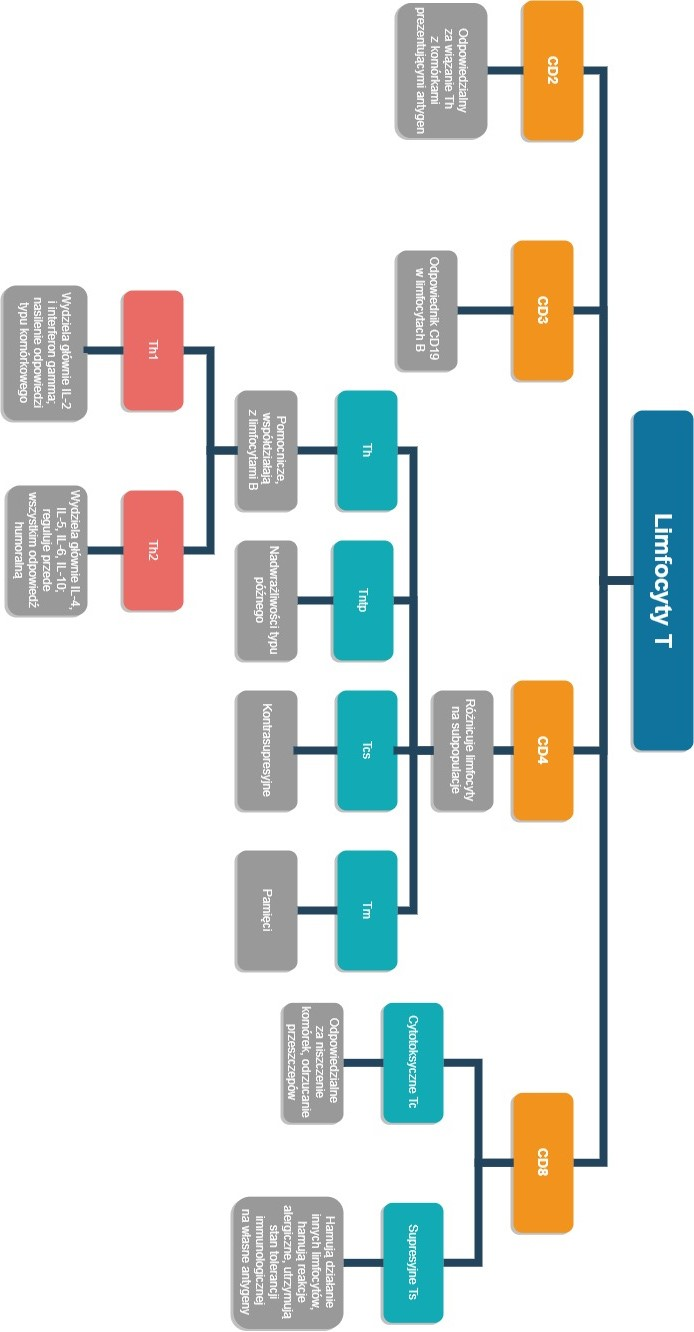
\includegraphics[width=0.7\textwidth]{Limf_TT2}
	\caption{Podzia� limfocyt�w typu T \cite{7}.}\label{limfocyty_T_cd8+} 
\end{figure}

% nowe p2
Podstaw� proces�w immunologicznych jest~prezentacja antygen�w przez~odpowiednie kom�rki pomocniczym limfocytom Th. Klasyczne kom�rki prezentuj�ce antygen APC (ang. Antigen Presenting Cells) to~limfocyty typu B, kom�rki dendryczne oraz~makrofagi. Natomiast, nieklasycznymi kom�rkami s�~limfocyty typu T, eozynofile, fibroblasty oraz~keranocyty \cite{7}.
% nowe k2

Odpowied� immunologiczna swoista typu kom�rkowego, w~kt�r� zaanga�owane s� subpopulacje limfocyt�w typu T, polega na~wywo�aniu reakcji zwalczania antygenu. Mo�liwe s� dwa typy tej reakcji. W~pierwszym z~nich funkcj� efektor�w pe�ni� limfocyty CD4+, a~makrofagi s� kom�rkami pomocniczymi. Drugi typ reakcji zak�ada, �e limfocyt cytotoksyczny CD8+ jest kom�rk� efektorow�, a~limfocyt CD4+ pomocnicz�.
Odporno�� kom�rkowa ma za~zadanie, przede wszystkim walczy� z~zaka�eniami, ale r�wnie� spe�nia wa�n� rol� w~reakcji kontaktowej ze zwi�zkami chemicznymi, w~ odrzuceniu przeszczepu czy~tkanek zmienionych nowotworowo i~w niekt�rych reakcjach autoimmunologicznych \cite{4}.
Mi�dzy 5 a~6 dekad� �ycia ustaje czynno�� grasicy, czego skutkiem s� zmiany w~subpopulacjach limfocyt�w typu T. Z~wiekiem g��wnie wzrasta liczba limfocyt�w CD4+, natomiast zmniejsza si� liczba limfocyt�w supresorowych i~cytotoksycznych CD8+ \cite{4}.

% nowe p3
Kom�rki nowotworowe wsp�dzia�aj�c~z~makrofagami TAMs M2 powoduj� immunosupresj�\footnote{Immunosupresja -- stan charakteryzuj�cy si� os�abieniem b�d�~zahamowaniem odpowiedzi immunologicznej; dotyczy zar�wno odpowiedzi typu humoralnego, jak i kom�rkowego. Wi��e si� ze~zmiennymi niedoborami poszczeg�lnych klas przeciwcia� (IgG, IgM, IgA) oraz~spadkiem liczby i~dysfunkcj� kom�rek uk�adu odporno�ciowego, g��wnie limfocyt�w T, ujawniaj�cym si� zahamowaniem wytwarzania cytokin \cite{26}.} uk�adu immunologicznego. W~pocz�tkowym etapie choroby mo�na zaobserwowa� wzrost poziomu cytokin prozapalnych. Czynniki te~hamuj� cytotoksyczn� aktywno�� makrofag�w. Kom�rki nowotworowe produkuj� r�wnie� cytokiny (IL-10, IL-4) stymuluj�ce polaryzacj� fenotypu w~kierunku klasy M2. Makrofagi TAMs M2 wydzielaj� zwi�zki o~dzia�aniu przeciwzapalnym, czego efektem jest~mi�dzy innymi indukcja limfocyt�w T regulatorowych ($T_{reg}$) oraz~supresja limfocyt�w $T_{CD8+}$ \cite{25}. Zwi�kszona ilo�� $T_{reg}$ hamuje aktywno�� kom�rek NK, TCD4+ i TCD8+, co~przyczynia si� do~rozrostu nowotworu \cite{27}.
% nowe p4

\newpage
\subsection{Kom�rki NK}
Swoj� rol� w~odpowiedzi immunologicznej maj� tak�e kom�rki NK, stanowi�ce populacj� odr�bn� od~limfocyt�w typu B~i~T. \cite{7}. K�m�rki NK stanowi� 10-15\% limfocyt�w obecnych we~krwi. Ich zadaniem jest niszczenie kom�rek nowotworowych i~zainfekowanych wirusami \cite{5}.

%nowe
Kom�rki NK to~efektorowe kom�rki cytotoksyczne b�d�ce elementem odporno�ci nieswoistej organizmu. S�~to du�e kom�rki limfoidalne posiadaj�ce umiej�tno�� rozpoznawania wielu konfiguracji molekularnych wyst�puj�cych m.in. na~kom�rkach w�asnych, zaka�onych wirusem oraz kom�rkach nowotworowych. Kom�rki NK s�~aktywowane, gdy~kom�rki  docelowe wykazuj� ekspresj� ligand�w wi���cych si� do~receptor�w kom�rek NK\cite{29}. \newline \newline \indent Kom�rki NK mog� wykazywa� ekspresj� r�nych receptor�w, np.\cite{29}:
\begin{itemize}
\item receptor�w naturalnej cytotoksyczno�ci NCRs (ang. Natural Cytotoxicity Receptors),
\item lektyno-podobnych receptor�w,
\item receptor�w aktywuj�cych czy~hamuj�cych kom�rki NK.
\end{itemize} 
%nowe

Charakterystyczn� cech� kom�rek NK jest brak posiadania marker�w czy~receptor�w antygenowych na~powierzchni. Dzia�anie kom�rek NK opiera si� na rozpoznawaniu przez receptor pektynowy reszt cukrowych, co umo�liwia im~cytotoksyczne zniszczenie kom�rki docelowej, mi�dzy innymi nowotworowej. Z~kolei receptor hamuj�cy kom�rki typu ,,zab�jcy'' KIR (ang. Killer cells Inhibitory Receptor) zmniejsza aktywno�� kom�rek NK, je�li rozpoznaj� one prawid�owe kom�rki organizmu \cite{4}.

Z wiekiem aktywno�� kom�rek NK spada (ze wzgl�du na~zwi�kszon� liczb� receptor�w KIR \cite{5}), co zwi�ksza ryzyko �mierci spowodowanej ci�k� infekcj�. Niekorzystnymi czynnikami maj�cymi wp�yw na~uk�ad kom�rek NK s�: stres, niska aktywno�� fizyczna oraz~dieta wysokot�uszczowa \cite{4}. Silna aktywno�� cytotoksyczna kom�rek NK mo�e by� uznana za~oznak� dobrego zdrowia \cite{5}.

\subsection{Interferony}
Interferony to~glikoproteiny wytwarzane przez limfocyty, fibroblasty i~inne kom�rki, kt�re bior� udzia� w~odpowiedzi immunologicznej \cite{21}. Nale�� do~humoralnych mechanizm�w obronnych odporno�ci nieswoistej. Ich funkcj� jest, mi�dzy innymi hamowanie replikacji wirus�w w~kom�rce i~proliferacji kom�rek (w szczeg�lno�ci nowotworowych), aktywowanie syntezy enzym�w (rybonukleazy, syntetazy, kinazy bia�kowej) i~cytotoksyczno�ci makrofag�w oraz~limfocyt�w typu T, a~tak�e zwi�kszenie aktywno�ci kom�rek cytotoksycznych \cite{7}.

W�r�d interferon�w mo�na wyr�ni� interferony \cite{22}:
\begin{itemize}
\item $\alpha$ (leukocytarne) � produkowane g��wnie przez monocyty, makrofagi i~limfocyty, zbudowane z~bia�ek zawieraj�cych od~165 do~166 aminokwas�w. Istniej� 22~znane podtypy interferon�w $\alpha$. S�~one~kodowane przez co~najmniej 23~geny zlokalizowane w~chromosomie 9;
\item $\beta$ � produkowane przez fibroblasty. S�~podobne do~interferon�w $\alpha$ (posiadaj� 30\% analogicznych aminokwas�w). Odpowiadaj�ce sobie geny interferon�w obu tych typ�w mieszcz� si� w~kr�tszym ramieniu chromosomu 9;
\item $\gamma$ � produkowane przez limfocyty typu T po~stymulacji antygenami lub~mitogenami. Gen koduj�cy interferony
$\gamma$ znajduje si� w~obr�bie chromosomu 12.
\end{itemize}

Warunkiem koniecznym do~dzia�ania interferon�w jest~ich~po��czenie ze~swoistymi receptorami. Interferony $\alpha$ i~$\beta$ dzia�aj� poprzez receptor typu I, natomiast interferon gamma poprzez receptor typu II. Liczba receptor�w r�ni si� zale�nie od~poszczeg�lnych kom�rek (waha si� od $2 \cdot 10^{2}$ do $6 \cdot 10^{3}$ \cite{22}). Kompleks interferon � receptor aktywuje kinaz� tyrozynow�. Poprzez fosforylacj� odpowiednich bia�ek kinaza tyrozynowa tworzy wraz z~nimi czynnik transkrypcyjny. W~j�drze kom�rkowym po~po��czeniu z~elementem odpowiedzi stymulowanej przez interferon ISRE (ang. Interferon-Stimulated Response Element) wzrasta ekspresja gen�w, kt�re s�~odpowiedzialne za produkcj� bia�ek efektorowych \cite{22}.

Interferon $\alpha$ (wykorzystywany, m. in. w procesie leczenia nowotwor�w) stymuluje uk�ad immunologiczny ingeruj�c w~procesy r�nicowania si� kom�rek. Zwi�ksza r�wnie� aktywno�� fagocytarn� makrofag�w i~swoiste dzia�anie cytotoksyczne limfocyt�w. Dzia�a przeciwnowotworowo poprzez hamowanie angiogenezy i~blokowanie syntezy bia�ek. W chorobach nowotworowych dawki interferonu dochodz� do 900 MU w ci�gu 6 dni \cite{21}.

Interferon posiada~wyra�ne powinowactwo do~kom�rek nerwowych i~w~du�ym st�eniu dzia�a neurotoksycznie. 
Podczas leczenia interferonem mog� wyst�pi� niepo��dane zaburzenia \cite{21}:

\begin{itemize}
\item uk�adu serotoninergicznego,
\item uk�adu noradrenergicznego,
\item uk�adu dopaminergicznego,
\item uk�adu glutaminianergicznego,
\item uk�adu opioidowego,
\item hormonalne,
\item metabolizmu m�zgowego.
\end{itemize}

Zaburzenia psychiczne cz�sto pojawiaj� si� u~pacjent�w leczonych przy~pomocy interferonu. Mog� to~by� stany zm�czenia, pogorszenie koncentracji, uwagi i~pami�ci, ale~tak�e pe�noobjawowe epizody depresji, manii, zaburzenia l�kowe czy zaburzenia �wiadomo�ci \cite{21}.

\subsection{Interleukiny}
Interleukiny s� jedn� z~grup cytokin\footnote{Cytokiny -- bia�ka o niskiej masie cz�steczkowej bior�ce udzia� w przekazywaniu informacji pomi�dzy kom�rkami; odgrywaj� istotn� rol� w odpowiedzi zapalnej, apoptozie, wzro�cie i r�nicowaniu kom�rek \cite{16}.}, kt�ra s�u�y, mi�dzy innymi do~komunikacji pomi�dzy kom�rkami uk�adu odporno�ciowego. Kom�rki te dotycz� zar�wno odporno�ci wrodzonej, jak~i~nabytej. Interleukiny to bia�ka produkowane g��wnie przez leukocyty. Ze wzgl�du na~cechy biologiczne, w~tym r�nice w~budowie molekularnej i~strukturze, interleukiny zosta�y zgrupowane w~trzy rodziny \cite{8}:
\begin{itemize}
\item pierwsz� -- podzielon� na~podrodzin� interleukiny-2 i~podrodzin� interferon�w (reprezentowan� przez interferon-$\alpha$ i~interferon-$\beta$),
\item drug� -- rodzin� interleukiny-1,
\item trzeci� -- zawieraj�c� interleukin� 17A, B, C, D, F oraz~IL-8, 25 i~27, a~tak�e IL-31, 32 i~33. 
\end{itemize}

\chapter{Sposoby leczenia nowotwor�w}
\section{Immunoterapia}

% nowe "Immunoonkologia nowe dane"
% nowe
Podczas immunoterapii dochodzi do~ingerencji w~uk�ad odporno�ciowy, co ma na~celu wzmocnienie lub~modyfikacj� mechanizm�w obronnych walcz�cych z~nowotworem. Immunoterapi� mo�na podzieli� na~biern� i~czynn� o~charakterze swoistym albo nieswoistym \cite{10}.

\subsection{Nieswoista bierna immunoterapia}
Nieswoista bierna immunoterapia ma za~zadanie wywo�a� nieswoist� aktywacj� uk�adu immunologicznego, a~w~konsekwencji dzia�anie przeciwnowotworowe na~skutek podawania m.in.~aktywowanych kom�rek efektorowych. Wykorzystuje si� tu, na~przyk�ad cytokiny czy~kom�rki zab�jcze aktywowane limfokin� LAK (ang. Lymphokine Activated Killers).
Aby wywo�a� efekt biologiczny konieczne jest po��czenie cytokiny ze swoistym receptorem na~kom�rkach docelowych (limfocytach typu T i~B, kom�rkach NK, monocytach, makrofagach i~granulocytach). Dzia�anie przeciwnowotworowe cytokin polega na:
\begin{itemize}
\item bezpo�rednim efekcie cytotoksycznym,
\item modyfikacji migracji limfocyt�w,
\item wzro�cie wra�liwo�ci kom�rek nowotworowych na~efekty cytotoksyczne r�nych czynnik�w biologicznych lub~chemicznych,
\item hamowaniu proliferacji kom�rek nowotworowych,
\item aktywacja kom�rek NK.
\end{itemize}
IFN-$\alpha$ to pierwsza rekombinowana cytokina zarejestrowana do~stosowania klinicznego \cite{10}.

\subsection{Swoista bierna immunoterapia}
Swoista bierna immunoterapia to metoda leczenia nowotworu, kt�ra polega na~podawaniu pacjentowi m.in.~kom�rek efektorowych swoi�cie ukierunkowanych na dan� kom�rk� nowotworow�. Do swoistej biernej immunoterapii zaliczamy \cite{10}:
\begin{itemize}
\item przeciwcia�a podawane przeciwko antygenom, kt�re wyst�puj� na~kom�rkach nowotworowych, 
\item terapie kom�rkowe, kt�re wykorzystuj� limfocyty naciekaj�ce guz (TIL); s� one izolowane, nast�pnie namno�one i~aktywowane, po czym ponownie przetaczane,
\item limfocyty krwi obwodowej stymulowane in vitro kom�rkami prezentuj�cymi antygen. 
\end{itemize} 

\subsection{Nieswoista czynna immunoterapia}
W nieswoistej czynnej immunoterapii pobudzany jest uk�ad odporno�ciowy, a~zw�aszcza odpowied� kom�rkowa. Wykorzystywane s� do~tego antygeny, niewyst�puj�ce w~kom�rkach nowotworu. Substancjami stymuluj�cymi procesy odporno�ciowe s� nieswoiste immunostymulatory (np. mikroorganizmy, elementy �ciany kom�rkowej) i~immunomodulatory (m. in. wyci�gi z~grasicy, syntetyczne hormony grasicy, tuftsyna, enkefaliny, endorfiny, wyci�gi z~limfocyt�w) \cite{10}.

\subsection{Swoista czynna immunoterapia}
Leczenie metod� swoistej czynnej immunoterapii polega na~pobudzaniu odporno�ci na~antygeny swoiste dla danego typu nowotworu. Wykorzystuje si� w~niej immunizacj� przy~u�yciu tzw. terapeutycznych szczepionek nowotworowych. S� to szczepionki:
\begin{itemize}
\item niekom�rkowe, na bazie bia�ek szoku cieplnego HSP (ang. Heat Shock Protein), szczepionki DNA oraz~szczepionki wirusowe,
\item kom�rkowe, niemodyfikowane i~modyfikowane genetycznie oraz~kom�rki dendrytyczne DC (ang. Dendritic Cells) �karmione� antygenami nowotworowymi \cite{10}.
\end{itemize}

\section{Chemioterapia}
Chemioterapia to metoda leczenia, kt�ra polega na~niszczeniu kom�rek nowotworowych, drobnoustroj�w oraz~bakterii za~pomoc� �rodk�w chemicznych. W~przypadku nowotwor�w, stosuje si� r�ne grupy lek�w, tzw. cytostatyk�w. Zale�nie od~indywidualnych cech pacjenta chemioterapia ma~�ci�le okre�lony przebieg. Leki mog� by� stosowane w~monoterapii (stosowanie jednego leku cytostatycznego) lub~polichemioterapii (stosowanie kilku lek�w zgodnie z~okre�lonym schematem). Leki cytostatyczne podawane s� w~sekwencjach co kilka dni, tygodni lub~stale, bez przerwy w~leczeniu. Leki cytostatyczne dzia�aj� w~okre�lonych fazach podzia�u kom�rek nowotworowych, zmniejszaj�c lub~spowalniaj�c ich~proliferacj�. Najcz�ciej podawane s� w~postaci do�ylnych wlew�w, lecz niekt�re z~nich maj� form� tabletek. Skutki uboczne chemioterapii mo�na zaobserwowa� ju�~po~kilku dniach terapii, a~czasem nawet po kilku godzinach \cite{9}. 

\section{Leczenie skojarzone}
Leczenie skojarzone polega na~po��czeniu u~pacjenta kilku metod leczenia nowotworu. Ten spos�b terapii posiada wiele zalet, mi�dzy innymi umo�liwia wykonanie zabiegu operacyjnego w~wielu przypadkach pierwotnie nieoperacyjnych i~pozwala zast�pi� okaleczaj�ce zabiegi chirurgiczne r�wnie skutecznym leczeniem zachowawczym. Ponadto, zmniejsza ryzyko wznowy miejscowej choroby i~rozwoju odleg�ych przerzut�w, co wp�ywa na~wyd�u�enie czasu prze�ycia chorych. 
Pomimo wielu zalet, leczenie skojarzone ma r�wnie� pewne wady, chocia�by, znaczne zwi�kszenie toksyczno�ci w~por�wnaniu z~monoterapi� czy~brak wsp�pracy mi�dzy specjalistami, co z~kolei utrudnia wdro�enie optymalnej terapii.

W�r�d metod leczenia skojarzonego mo�na wyr�ni� \cite{11}:
\begin{itemize}
\item leczenie sekwencyjne -- poszczeg�lne metody lecznicze stosowane jedna po~drugiej, np.:
\begin{itemize}
\item[-] leczenie wst�pne (neoadiuwantowe, indukcyjne) � poprzedza leczenie radykalne. Jego celem jest wczesne oddzia�ywanie na~mikroprzerzuty lub~zmniejszenie masy guza u~chorych z~miejscowo zaawansowanym nowotworem i~umo�liwienie tym samym przeprowadzenia leczenia radykalnego;
\item[-] uzupe�niaj�ce (adiuwantowe) � stosowane jest po leczeniu radykalnym, czyli u~os�b bez cech choroby nowotworowej. Jego celem jest zniszczenie potencjalnie istniej�cych mikroprzerzut�w i~zmniejszenie tym samym prawdopodobie�stwa nawrotu nowotworu;
\end{itemize}
\item leczenie r�wnoczesne � kojarzenie r�nych metod
leczenia w~tym samym czasie, na~przyk�ad r�wnoczesna
chemioradioterapia oraz napromienianie �r�doperacyjne;
\item leczenie naprzemienne � dotyczy kojarzenia radioterapii
i chemioterapii.
\end{itemize}

W tej pracy omawiany jest przypadek leczenia skojarzon� metod� chemioterapii i~immunoterapii, zwanej tak�e biochemioterapi� \cite{1}.

\chapter{Model matematyczny}

Model matematyczny wykorzystany w~pracy to~model b�d�cy po��czeniem modelu de Pillis'a \cite{19} oraz~modelu Isaeva i~Osipov'a \cite{18} opisany w~literaturze \cite{1}. W~pierwszym etapie rozwa�ymy model bez uwzgl�dnienia procesu leczenia, kt�ry obejmuje cztery populacje kom�rek, tj.:
\begin{itemize}
\item $\mathcal{T}$ -- populacj� kom�rek nowotworowych,
\item $\mathcal{N}$ -- populacj� kom�rek NK,
\item $\mathcal{L}$ -- populacj� limfocyt�w $T_{CD8+}$,
\item $\mathcal{C}$ -- populacj� limfocyt�w kr���cych,
\end{itemize}

W drugim etapie model zostaje poddany modyfikacji, uwzgl�dnia proces leczenia i~dodatkowo badane s� zmiany st�enia w~czasie trzech podawanych lek�w:
\begin{itemize}
\item $I(t)$ -- funkcja st�enia interleukin-2 w~czasie,
\item $I_{\alpha}$(t) -- funkcja st�enia interferon�w-$\alpha$ w~czasie,
\item $M(t)$ -- funkcja st�enia cytostatyku u�ytego w~chemioterapii w~czasie.
\end{itemize}

W r�wnaniach modelu przed~modyfikacj� uwzgl�dniono takie czynniki, jak:
\begin{itemize}
\item naturalny rozw�j i~�mier� kom�rek,
\item �mier� kom�rek nowotworowych pod wp�ywem kom�rek NK, limfocyt�w $T_{CD8+}$,
\item wytwarzanie kom�rek NK i~limfocyt�w $T_{CD8+}$,
\item dezaktywacj� kom�rek NK i~limfocyt�w $T_{CD8+}$.
\end{itemize}

Natomiast w~modelu zmodyfikowanym wzi�to pod~uwag� r�wnie�:
\begin{itemize}
\item ilo�� podawanych lek�w i~czas, w~kt�rym zosta�y podane,
\item �mier� kom�rek nowotworowych pod wp�ywem podawanych lek�w.
\end{itemize}

\section{Model nieuwzgl�dniaj�cy procesu leczenia}
\subsection{Za�o�enia modelu} \label{zalozenia}

Przyj�to za�o�enia jak~w~modelu de Pillis'a, Isaeva i~Osipov'a \cite{1}:
\begin{enumerate}
\item W~przypadku braku odpowiedzi uk�adu immunologicznego liczba kom�rek nowotworowych wzrasta logistycznie.
\item Kom�rki NK i~limfocyty $T_{CD8+}$ s� zdolne zniszczy� kom�rki nowotworu.
\item Pod wp�ywem kom�rek nowotworowych kom�rki NK i~limfocyty $T_{CD8+}$ ulegaj� szybszej proliferacji oraz~wzrasta ich aktywno�� cytolityczna\footnote{Aktywno�� cytolityczna -- jeden z~mechanizm�w cytotoksyczno�ci limfocyt�w s�u��cy do~niszczenia kom�rek zainfekowanych lub~nowotworowych \cite{15}.}.
\item Kom�rki NK s� zawsze obecne w~organizmie, tak�e w~przypadku braku wyst�powania kom�rek nowotworowych.
\item W~organizmie wyst�puje du�a liczba aktywnych limfocyt�w $T_{CD8+}$, tylko w~przypadku obecno�ci kom�rek nowotworowych. Jest to specyficzna odpowied� immunologiczna.
\item Kom�rki NK i~limfocyty $T_{CD8+}$ ulegaj� ca�kowitej dezaktywacji po pewnej liczbie interakcji z~kom�rkami nowotworowymi.
\item Kom�rki nowotworowe dezaktywuj� si� pod wp�ywem interferon�w $\alpha$.
\item Poziom kr���cych limfocyt�w mo�e s�u�y� do~oceny zdrowia pacjenta.
\item Odsetek kom�rek nowotworowych zniszczonych w~wyniku chemioterapii zale�y od~ilo�ci cytostatyku obecnego w~organizmie. Maksymalny odsetek zniszczonych kom�rek wynosi mniej ni� 1 ze~wzgl�du na~to,�e~pokonanie kom�rek nowotworowych wskutek chemioterapii jest mo�liwe tylko na~niekt�rych etapach ich rozwoju.
\item Cz�� kom�rek NK, limfocyt�w $T_{CD8+}$ i~limfocyt�w kr���cych jest niszczona podczas chemioterapii.
\item Kom�rki NK i~limfocyty $T_{CD8+}$ uczestnicz� w~procesie stymulacji i~eliminacji aktywowanych kom�rek (efektor�w); uproszczony model ma odzwierciedla� samoreguluj�cy si� charakter uk�adu immunologicznego.
\end{enumerate}

\newpage
\subsection{R�wnania i opis modelu}

W~modelu nieleczonego guza, rozwa�amy cztery populacje kom�rek, s�~to~populacja kom�rek nowotworowych ($\mathcal{T}$), populacja kom�rek NK ($\mathcal{N}$), populacja limfocyt�w $T_{CD8+}$ ($\mathcal{L}$) oraz~populacja limfocyt�w kr���cych ($\mathcal{C}$). \newline \newline Model nieleczonego guza nowotworowego jest uk�adem r�wna� r�niczkowych zwyczajnych \ref{r�wnania_modelu_pillis_i_isaeva_bez_leczenia}. R�wnania tego modelu przedstawiaj� tempo zmian proliferacji kom�rek nowotworowych oraz~tempo zmian liczby kom�rek uk�adu immunologicznego (kom�rek NK, limfocyt�w $T_{CD8+}$ oraz~limfocyt�w kr���cych) w~odpowiedzi na~wzrost liczby kom�rek nowotworowych.\newline \newline

\begin{equation}
\label{r�wnania_modelu_pillis_i_isaeva_bez_leczenia}
\left\{ \begin{array}{ll}
\dfrac{dT}{dt}=aT(1-bT)-cNT-DT,\\\\
\dfrac{dN}{dt}=eC-fN+g\dfrac{T^{2}}{h+T^{2}}N-pNT,\\\\
\dfrac{dL}{dt}=-mL+j\dfrac{D^{2}T^{2}}{k+D^{2}T^{2}}L-qLT+(r_{1}N+r_{2}C)T-uNL^{2},\\\\
\dfrac{dC}{dt}=\alpha-\beta C,\\\\
\end{array} \right.
\end{equation}

gdzie: 
\begin{itemize}
\item T(t) - liczba kom�rek nowotworowych w chwili czasowej t,
\item N(t) - liczba kom�rek NK w chwili czasowej t,
\item L(t) - liczba limfocyt�w $T_{CD8+}$ w chwili czasowej t,
\item C(t) - liczba limfocyt�w kr���cych w chwili czasowej t,
\item $D=d\dfrac{(\frac{L}{T})^{l}}{s+(\frac{L}{T})^{l}}$ - liza nowotworu pod~wp�ywem dzia�ania limfocyt�w $T_{CD8+}$.
\end{itemize}

\noindent \newline Pierwsze z~r�wna� modelu \ref{r�wnania_modelu_pillis_i_isaeva_bez_leczenia} opisuje tempo zmian $\dfrac{dT}{dt}$ liczby kom�rek nowotworowych, w~chwili czasowej t, uwzgl�dniaj�c zar�wno proces proliferacji tych kom�rek, jak~i~efekt cytotoksyczno�ci wywo�any odpowiedzi� uk�adu immunologicznego.
\newline Wyra�enie $aT(1-bT)$ zwi�ksza pr�dko�� zmian liczebno�ci populacji kom�rek nowotworowych, gdy� okre�la liczb� kom�rek nowotworowych, kt�re powsta�y w~danej chwili czasowej t w~wyniku ich~proliferacji. Wyra�enia $-cNT$ oraz~$-DT$ z~kolei hamuj� tempo zmian liczebno�ci kom�rek nowotworowych, gdy� przedstawiaj� odpowiednio: liczb� kom�rek nowotworowych zniszczonych na~skutek ich~interakcji z~kom�rkami NK oraz~z~limfocytami $T_{CD8+}$, w~danej chwili czasowej t. 

Drugie r�wnanie modelu \ref{r�wnania_modelu_pillis_i_isaeva_bez_leczenia} okre�la tempo zmian $\dfrac{dN}{dt}$ liczebno�ci populacji kom�rek NK, w~chwili czasowej t, na~kt�re wp�ywa kilka sk�adnik�w. \newline Sk�adnik $eC$ to~liczba kom�rek NK powsta�ych z~kr���cych limfocyt�w w~chwili czasowej t, $-fN$ opisuje liczb� kom�rek NK zniszczonych w~chwili czasowej t. \newline Sk�adowa $g\dfrac{T^{2}}{h+T^{2}}N$ okre�la liczb� nowopowsta�ych kom�rek okre�lonych jako NK w~chwili czasowej t, natomiast $-pNT$ to~kom�rki NK dezaktywowane w~chwili czasowej t na~skutek interakcji z~kom�rkami nowotworowymi.

Trzecim r�wnaniem modelu \ref{r�wnania_modelu_pillis_i_isaeva_bez_leczenia} zosta�o opisane tempo zmian liczebno�ci populacji limfocyt�w $T_{CD8+}$ $\dfrac{dL}{dt}$. \newline Pierwsza sk�adowa $-mL$ okre�la liczb� limfocyt�w $T_{CD8+}$ zniszczonych w~chwili czasowej t na~skutek obecno�ci kom�rek nowotworowych. Kolejna $j\dfrac{D^{2}T^{2}}{k+D^{2}T^{2}}L$ to~liczba limfocyt�w $T_{CD8+}$ stymulowanych przez kom�rki nowotworowe, kt�re s�~lizowane przez limfocyty $T_{CD8+}$  w~chwili czasowej t. Liczba dezaktywowanych limfocyt�w $T_{CD8+}$ w~chwili czasowej t na~skutek interakcji z~kom�rkami nowotworowymi jest~opisana przy~pomocy sk�adowej $-qLT$. Przedostatni� sk�adow� w~tym r�wnaniu jest~$(r_{1}N+r_{2}C)T$ odpowiadaj�ca liczbie limfocyt�w $T_{CD8+}$ stymulowanych przez kom�rki nowotworowe, kt�re s�~lizowane przez kom�rki NK oraz~limfocyt�w $T_{CD8+}$ powsta�ych na~skutek obecno�ci kom�rek nowotworowych w~chwili czasowej t. $-uNL^{2}$ wyznacza liczb� limfocyt�w $T_{CD8+}$ dezaktywowanych w~chwili czasowej t na~skutek dzia�ania kom�rek NK.

R�wnanie czwarte okre�la tempo zmian liczebno�ci populacji limfocyt�w kr���cych $\dfrac{dC}{dt}$,w~chwili czasowej t, kt�re jest modulowane poprzez r�nic� mi�dzy sta�� liczb� $\alpha$ kr���cych limfocyt�w a stopniem ich degradacji $-\beta C$, gdzie $\beta$ to~sta�a okre�laj�ca tempo wyniszczania kr���cych limfocyt�w.

\begin{table}[h]
\caption{Parametry modelu odpowiedzi immunologicznej na~rozwijaj�cy si� nowotw�r bez uwzgl�dnienia procesu leczenia.}\label{parametry_modelu}
	\centering
	\begin{tabular}{|c|c|c|p{0.47\linewidth}|} \hline \hline
		Nazwa & Warto�� & Jednostka & Opis  \\ \hline
		a & $4,31 \cdot 10^{-1}$ & dzie�$^{-1}$ & Tempo wzrostu nowotworu \\ \hline
		b & $1,02 \cdot 10^{-9}$ & kom�rka$^{-1}$ & Odwrotno�� pojemno�ci �rodowiska \\ \hline
		c & $6,41 \cdot 10^{-11}$ & dzie�$^{-1} \cdot$ kom�rka$ ^{-1}$ & Liczba kom�rek nowotworu zabita przez kom�rki NK \\ \hline
		d & $2,34$ &  dzie�$^{-1}$ & Wsp�czynnik si�y uk�adu odporno�ciowego \\ \hline
		e & $2,08 \cdot 10^{-7}$ & dzie�$^{-1}$ & Liczba kr���cych limfocyt�w, kt�re sta�y si� kom�rkami NK \\ \hline
		l & $2,9$ & bezwymiarowe & Wsp�czynnik skalowania si�y uk�adu odporno�ciowego \\ \hline
		f & $4,12 \cdot 10^{-2}$ & dzie�$^{-1}$ & Tempo wyniszczania kom�rek NK \\ \hline
		g & $1,25 \cdot 10^{-2}$ & dzie�$^{-1}$ & Maksymalna liczba kom�rek NK wytwarzanych na~skutek obecno�ci kom�rek nowotworowych \\ \hline
		h & $2,02 \cdot 10^{7}$ & kom�rka$^{2}$ & Wsp�czynnik stromo�ci krzywej rekrutacji kom�rek NK \\ \hline
		j & $2,49 \cdot 10^{-2}$ & dzie�$^{-1}$ & Maksymalne tempo rekrutacji limfocyt�w $T_{CD8+}$ \\ \hline
		k & $3,66 \cdot 10^{7}$ & kom�rka$^{2}$ & Wsp�czynnik stromo�ci krzywej rekrutacji limfocyt�w $T_{CD8+}$ \\ \hline
		m & $2,04 \cdot 10^{-1}$ & dzie�$^{-1}$ & Tempo wyniszczania limfocyt�w $T_{CD8+}$ \\ \hline
		q & $1,42 \cdot 10^{-6}$ & dzie�$^{-1} \cdot$ kom�rka$^{-1}$ & Tempo dezaktywacji limfocyt�w $T_{CD8+}$ przez kom�rki nowotworu \\ \hline
		p & $3,42 \cdot 10^{-6}$ & dzie�$^{-1} \cdot$ kom�rka$^{-1}$ & Tempo dezaktywacji kom�rek NK przez kom�rki nowotworu \\ \hline
		s & $8,39 \cdot 10^{-2}$ & bezwymiarowe & Warto�� ${(\frac{L}{T})}^{l}$ konieczna do~osi�gni�cia po�owy maksymalnej warto�ci cytotoksyczno�ci limfocyt�w $T_{CD8+}$\\ \hline
		$r_{1}$ & $1,1 \cdot 10^{-7}$ & dzie�$^{-1} \cdot$ kom�rka$^{-1}$ & Tempo stymulacji wytwarzania limfocyt�w $T_{CD8+}$ jako rezultat niszczenia kom�rek nowotworowych przez kom�rki NK \\ \hline
		$r_{2}$ & $6,5 \cdot 10^{-11}$ & kom�rka$^{-1} \cdot$ dzie�$^{-1}$ & Tempo stymulacji wytwarzania limfocyt�w $T_{CD8+}$ jako rezultat interakcji kom�rek  nowotworowych z~kr���cymi limfocytami \\ \hline
		u & $3 \cdot 10^{-10}$ & kom�rka$^{-2} \cdot$ dzie�$^{-1}$ &  Wsp�czynnik Funkcji regulacyjnej limfocyt�w $T_{CD8+}$ nadzorowanej przez kom�rki NK\\ \hline
		$\alpha$ & $7,5 \cdot 10^{8}$ & kom�rka $\cdot$ dzie�$^{-1}$ &  Sta�a liczba kr���cych limfocyt�w\\ \hline
		$\beta$ & $1,2 \cdot 10^{-2}$ & dzie�$^{-1}$ & Tempo wyniszczania kr���cych limfocyt�w\\ \hline
		\end{tabular}
\end{table}

\section{Model uwzgl�dniaj�cy proces leczenia}

Przyj�to za�o�enia dla~modelu jak w~rozdziale \ref{zalozenia}.
 
\subsection{R�wnania i opis modelu}

W~modelu \ref{r�wnania_modelu_pillis_i_isaeva_z_leczeniem}, poza czterema populacjami uwzgl�dnionymi w modelu \ref{r�wnania_modelu_pillis_i_isaeva_bez_leczenia}, rozwa�amy dodatkowo zmiany st�enia trzech podawanych lek�w, czyli interleukin-2 ($I$), interferon�w-$\alpha$ ($I_{\alpha}$) oraz cytostatyku u�ytego w~chemioterapii ($M$). \newline \newline Przedstawione w~uk�adzie \ref{r�wnania_modelu_pillis_i_isaeva_z_leczeniem} r�wnania okre�laj� tempo zmian liczebno�ci populacji, jak w~modelu \ref{r�wnania_modelu_pillis_i_isaeva_bez_leczenia}, ale~tak�e opisuj� wp�yw podawanych lek�w na~nowotw�r oraz~ich~rozpad w~organizmie. Modyfikacje wprowadzone do~modelu, odpowiadaj�ce podawanym lekom zaznaczono w~uk�adzie \ref{r�wnania_modelu_pillis_i_isaeva_z_leczeniem} na~czerwono. \newline \newline Parametry modelu leczonego guza \ref{r�wnania_modelu_pillis_i_isaeva_z_leczeniem}, ukazano w~tabeli \ref{parametry_modelu_z}.

\begin{equation}
\label{r�wnania_modelu_pillis_i_isaeva_z_leczeniem}
\left\{ \begin{array}{ll}
\dfrac{dT}{dt}=aT(1-bT)-cNT-DT \textcolor{red}{-K_{T}(1-e^{-M})T - c'TL},\\\\
\dfrac{dN}{dt}=eC-fN+g\dfrac{T^{2}}{h+T^{2}}N-pNT \textcolor{red}{-K_{N}(1-e^{-M})N},\\\\
\dfrac{dL}{dt}=-mL+j\dfrac{D^{2}T^{2}}{k+D^{2}T^{2}}L-qLT+(r_{1}N+r_{2}C)T-uNL^{2} \textcolor{red}{-K_{L}(1-e^{-M})L+\dfrac{p_{i}LI}{g_{i}}+ \nu_{L}(t)},\\\\
\dfrac{dC}{dt}=\alpha-\beta C \textcolor{red}{-K_{C}(1-e^{-M})C},\\\\
\textcolor{red}{ \dfrac{dM}{dt}=-\gamma M+\nu_{M}(t)},\\\\
\textcolor{red}{ \dfrac{dI}{dt}=-\mu_{i}I-j'LI-k'TI+\nu_{I}(t)},\\\\
\textcolor{red}{ \dfrac{dI_{\alpha}}{dt}=\nu_{\alpha}(t)-g'I_{\alpha}},\\\\
\end{array} \right.
\end{equation}

gdzie: 
\begin{itemize}
\item T(t) - liczba kom�rek nowotworowych w chwili czasowej t,
\item N(t) - liczba kom�rek NK w chwili czasowej t,
\item L(t) - liczba limfocyt�w $T_{CD8+}$ w chwili czasowej t,
\item C(t) - liczba limfocyt�w kr���cych w chwili czasowej t,
\item \textcolor{red}{M(t) - st�enie cytostatyku w chwili czasowej t},
\item \textcolor{red}{I(t) - st�enie interleukin-2 w chwili czasowej t},
\item \textcolor{red}{$I_{\alpha}$(t) - st�enie interferon�w-$\alpha$ w chwili czasowej t},
\item $D=d\dfrac{(\frac{L}{T})^{l}}{s+(\frac{L}{T})^{l}}$ - liza nowotworu pod~wp�ywem dzia�ania limfocyt�w $T_{CD8+}$,
\item \textcolor{red}{$c'=c_{CTL}(2-e^{\frac{I_{\alpha}}{I_{\alpha 0}}})$} - wp�yw st�enia interferon�w-$\alpha$ na~rozpoznawanie kom�rek nowotworowych przez~limfocyty $T_{CD8+}$.
\end{itemize}

\begin{table}[!h]
\caption{Dodatkowe parametry modelu odpowiedzi immunologicznej na~rozwijaj�cy si� nowotw�r z uwzgl�dnieniem procesu leczenia.}\label{parametry_modelu_z}
	\centering
	\begin{tabular}{|c|c|c|p{0.49\linewidth}|} \hline 
		$\gamma$ & $9 \cdot 10^{-1}$ & dzie�$^{-1}$ & Tempo rozpadu leku chemioterapeutycznego \\ \hline
		$p_{i}$ & $1,25 \cdot 10^{-1}$ & dzie�$^{-1}$ & Maksymalne tempo rekrutacji limfocyt�w $T_{CD8+}$ przez interleukiny-2 \\ \hline
		$g_{i}$ & $2 \cdot 10^{2}$ & kom�rka$^{2}$ & Warto�� st�enia interleukiny-2 konieczna do~osi�gni�cia po�owy maksymalnej warto�ci aktywno�ci cytolitycznej limfocyt�w $T_{CD8+}$ \\ \hline
		$\mu_{i}$ & $1 \cdot 10^{1}$ & dzie�$^{-1}$ & Tempo rozpadu interleukiny-2 (leku) \\ \hline
		$C_{CTL}$ & $4,4 \cdot 10^{-9}$ & kom�rka$^{-1} \cdot$ dzie�$^{-1}$ & Tempo dezaktywacji nowotworu przez limfocyty $T_{CD8+}$ \\ \hline
		g' & $1,7$ & dzie�$^{-1}$ & Tempo rozpadu terapeutycznego interferonu-$\alpha$\\ \hline
		j' & $3,3 \cdot 10^{-9}$ & kom�rka$^{-1} \cdot$ dzie�$^{-1}$ & Tempo wch�aniania interleukiny-2 przez limfocyty $T_{CD8+}$ \\ \hline
		k' & $1,8 \cdot 10^{-8}$ & kom�rka$^{-1} \cdot$ dzie�$^{-1}$ & Dezaktywacja moleku� interleukiny-2 przez prostaglandyny \\ \hline
		\multicolumn{2}{|l|}{$I_{\alpha 0}$} & jednostki & Pocz�tkowa ilo�� interferonu-$\alpha$ \\ \hline		
	\end{tabular}
\end{table}

\noindent
W~odr�nieniu od~modelu \ref{r�wnania_modelu_pillis_i_isaeva_bez_leczenia}, w~ pierwszym r�wnaniu modelu \ref{r�wnania_modelu_pillis_i_isaeva_z_leczeniem} wyst�puje dodatkowo sk�adowa $-K_{T}(1-e^{-M})T$, kt�ra opisuje liczb� kom�rek nowotworowych zniszczonych w~danej chwili czasowej t na~skutek dzia�ania cytostatyku podanego podczas chemioterapii. Kolejn� modyfikacj� jest $-c'TL$, opisuj�ca liczb� kom�rek nowotworowych zniszczonych w~danej chwili czasowej t na~skutek interakcji pomi�dzy IFN-$\alpha$, limfocytami $T_{CD8+}$ i~kom�rkami nowotworu.

\noindent \newline W~drugim r�wnaniu modele \ref{r�wnania_modelu_pillis_i_isaeva_bez_leczenia} i~\ref{r�wnania_modelu_pillis_i_isaeva_z_leczeniem} r�ni� si� tylko sk�adow� $-K_{N}(1-e^{-M})N$ okre�laj�c� liczb� kom�rek NK zniszczonych w~chwili czasowej t na~skutek dzia�ania cytostatyku podanego podczas chemioterapii.

\noindent \newline Trzecie r�wnanie modelu \ref{r�wnania_modelu_pillis_i_isaeva_z_leczeniem}, poza wyja�nionymi wcze�niej sk�adowymi okre�la tak�e $-K_{L}(1-e^{-M})L$ - liczb� limfocyt�w $T_{CD8+}$ zniszczonych w~chwili czasowej t na~skutek dzia�ania cytostatyku podanego podczas chemioterapii oraz $\dfrac{p_{i}LI}{g_{i}}$ - liczb� limfocyt�w $T_{CD8+}$ stymulowanych przez IL-2. Funkcj� opisuj�c� ilo�� i~czas podania TIL jest $\nu_{L}(t)$.

\noindent \newline Jedyn� zmian� w~r�wnaniu czwartym w~stosunku do modelu \ref{r�wnania_modelu_pillis_i_isaeva_bez_leczenia} jest~wprowadzenie sk�adowej $-K_{C}(1-e^{-M})C$ wyznaczaj�cej liczb� limfocyt�w kr���cych zniszczonych w~chwili czasowej t na~skutek dzia�ania cytostatyku podanego podczas chemioterapii.

\noindent \newline \newline W~modelu leczonego guza \ref{r�wnania_modelu_pillis_i_isaeva_z_leczeniem} dodano kolejne trzy r�wnania r�niczkowe opisuj�ce tempo zmian st�e� podawanych lek�w.

\noindent \newline R�wnanie pi�te okre�la zmiany st�enia cytostatyku w~organizmie $\dfrac{dM}{dt}$. Sk�adowa $-\gamma M$ odpowiada spadkowi st�enia cytostatyku na~skutek jego rozpadu, a~$\nu_{M}(t)$ to~wyra�enie opisuj�ce ilo�� i~czas podania cytostatyku.

\noindent \newline Kolejne r�wnanie uk�adu okre�la tempo zmian st�enia IL-2 w~organizmie $\dfrac{dI}{dt}$. Spadek st�enia IL-2 na~skutek jej rozpadu okre�la sk�adowa $-\mu_{i}L$. $-j'LI$ jest~liczb� kom�rek IL-2 wch�oni�tych przez limfocyty $T_{CD8+}$ w~chwili czasowej t, natomiast $-k'TI$, liczb� kom�rek IL-2 dezaktywowanych przez prostaglandyny w~chwili czasowej t. $\nu_{I}(t)$ to~funkcja opisuj�ca ilo�� i~czas podania IL-2.

\noindent \newline W~si�dmym r�wnaniu okre�lone jest~tempo zmian st�enia IFN-$\alpha$ w~organizmie $\dfrac{dI_{\alpha}}{dt}$. $-gI_{\alpha}$ okre�la spadek st�enia IFN-$\alpha$ na~skutek jego rozpadu, a~$\nu_{\alpha}(t)$ jest~funkcj� opisuj�c� ilo�� i~czas podania IFN-$\alpha$.

\chapter{Symulacje}
W pracy przeprowadzono modelowanie odpowiedzi uk�adu immunologicznego na~rozwijaj�cy si� nowotw�r:
\begin{itemize}
\item bez uwzgl�dnienia procesu leczenia,
\item z~uwzgl�dnieniem leczenia wy��cznie metod� chemioterapii,
\item z~uwzgl�dnieniem leczenia wy��cznie metod� immunoterapii,
\item z~uwzgl�dnieniem leczenia skojarzonymi metodami chemioterapii i~immunoterapii.
\end{itemize}

Warunki pocz�tkowe (Tab. \ref{warunki_poczatkowe_bez}) dla modelu \ref{r�wnania_modelu_pillis_i_isaeva_bez_leczenia} dobrano zgodnie z~literatur� \cite{1}. Dla~wi�kszej czytelno�ci, wielko�� nowotworu okre�lono r�wnie� poprzez d�ugo�� jego~promienia, przyjmuj�c, �e~nowotw�r ma~kszta�t zbli�ony do~kuli, a~na~1~cm$^{3}$ przypada $10^{9}$ kom�rek \cite{23}.

\begin{table}[!htb]
\caption{Warunki pocz�tkowe dla modelu odpowiedzi immunologicznej na~rozwijaj�cy si� nowotw�r bez uwzgl�dnienia procesu leczenia.}\label{warunki_poczatkowe_bez}
	\centering
	\begin{tabular}{|c|c|c|} \hline \hline
		Warto�� [liczba kom�rek] & Rodzaj kom�rek & Promie� nowotworu [mm]\\ \hline
		$T(0) = 1 \cdot 10^{6}$ & Kom�rki nowotworowe & 0,62 \\ \hline
		$N(0) = 1 \cdot 10^{5}$  & Kom�rki NK \\ \cline{1-2}
		$L(0) = 1 \cdot 10^{2}$ & Limfocyty $T_{CD8+}$ \\ \cline{1-2}
		$C(0) = 6 \cdot 10^{10}$ & Limfocyty kr���ce \\ \cline{1-2}
		\end{tabular}
\end{table}

\newpage
\section{Odpowied� uk�adu immunologicznego na~rozwijaj�cy si� w~organizmie nowotw�r -- brak leczenia}
%\setlength{\parindent}{0pt}
%\noindent % brak akapitu
\subsection{Scenariusz I -- symulacja wykonana dla modelu nieleczonego guza}

\noindent \textbf{Podejmowany problem:} \newline Analiza zmian odpowiedzi uk�adu immunologicznego w~zale�no�ci od~pocz�tkowej wielko�ci nowotworu (na~podstawie wielko�ci nowotworu po zadanym czasie symulacji).

\noindent \newline \textbf{Warunki pocz�tkowe:} \newline Wielko�� (tj., liczb� kom�rek) nowotworu $T(0)$, liczb� kom�rek NK $N(0)$, liczb� limfocyt�w $T_{CD8+}$ oraz~liczb� limfocyt�w kr���cych $C(0)$ dobrano jak~w~tabeli \ref{warunki_poczatkowe_bez}, a~nast�pnie do�wiadczalnie zmieniano warto�� pocz�tkowej wielko�ci nowotworu $T(0)$.

\noindent \newline \textbf{Przyj�te parametry:} \newline Parametry dla~modelu nieuwzgl�dniaj�cego leczenia jak~w~tabeli \ref{parametry_modelu}.

\noindent \newline \textbf{Czas symulacji:} \newline $T_{k}$ = 120 dni \newline \newline W tabeli \ref{zmiany_poczatkowej_wartosci_T} przedstawiono pocz�tkow� liczb� kom�rek nowotworu $T(0)$, liczb� kom�rek nowotworu po~symulacji w~chwili $T_{k}$ = 120 dni $T(120)$ oraz~szacowan� obj�to�� i~d�ugo�� promienia nowotworu po~symulacji w~chwili $T_{k}$ = 120 dni.

\begin{table}[!htb]
\caption{Pocz�tkowa liczba kom�rek nowotworowych $T(0)$, liczba kom�rek nowotworowych po~symulacji w~chwili $T_{k}$ = 120 dni $T(120)$ oraz~szacowana obj�to�� i~d�ugo�� promienia nowotworu po~symulacji w~chwili $T_{k}$ = 120 dni.}\label{zmiany_poczatkowej_wartosci_T}
	\centering
\begin{tabular}{|c|c|c|c|} \hline \hline
		$T(0)$ & $T(120)$ & Obj�to�� & Promie� \\
		$[$liczba kom�rek$]$ & $[$liczba kom�rek$]$ & nowotworu [$mm^{3}$] & nowotworu [$mm$] \\ \hline
		$1 \cdot 10^{6}$ & $6,76 \cdot 10^{-8}$ & $6,76 \cdot 10^{-14}$ & $2,5 \cdot 10^{-5}$ \\ \hline
		$2 \cdot 10^{6}$ & $8,15 \cdot 10^{-8}$ & $8,15 \cdot 10^{-14}$ & $2,7 \cdot 10^{-5}$ \\ \hline
		$5 \cdot 10^{6}$ & $2,69 \cdot 10^{-8}$ & $2,69 \cdot 10^{-14}$ & $1,9 \cdot 10^{-5}$ \\ \hline
		$1 \cdot 10^{7}$ & $3,44 \cdot 10^{-8}$ & $3,44 \cdot 10^{-14}$ & $2 \cdot 10^{-5}$ \\ \hline
		$1,5 \cdot 10^{7}$ & $4,41 \cdot 10^{-8}$ & $4,41 \cdot 10^{-14}$ & $2,2 \cdot 10^{-5}$ \\ \hline
		$1,7 \cdot 10^{7}$ & $2,96 \cdot 10^{-8}$ & $2,96 \cdot 10^{-14}$ & $1,9 \cdot 10^{-5}$ \\ \hline
		$1,75 \cdot 10^{7}$ & $3,67 \cdot 10^{-8}$ & $3,67 \cdot 10^{-14}$ & $2,1 \cdot 10^{-5}$ \\ \hline
		$1,8 \cdot 10^{7}$ & $9,8 \cdot 10^{8}$ & $980$ & $6,16$ \\ \hline
		$2 \cdot 10^{7}$ & $9,8 \cdot 10^{8}$ & $980$ & $6,16$ \\ \hline
		$5 \cdot 10^{7}$ & $9,8 \cdot 10^{8}$ & $980$ & $6,16$ \\ \hline
		\end{tabular}
\end{table}

Przyk�adowe zmiany liczby kom�rek ka�dej z~czterech badanych populacji - kom�rek nowotworowych $T(t)$, kom�rek NK $N(t)$, limfocyt�w $T_{CD8+}$ $L(t)$ i~limfocyt�w kr���cych $C(t)$ przedstawiono na~poni�szych wykresach (Rys. \ref{zmiany_liczby_kom_4_populacji}). 

\begin{figure}
\centering
\subfloat[Zmiany liczby kom�rek badanych populacji dla~warto�ci pocz�tkowej liczby kom�rek nowotworowych $T(0) = 1 \cdot 10^{6}$. Regresja nowotworu po~czasie $T_{r}$~$\approx$ 7 dni (168 godzin).]{\label{bez_lecz_stlumienie}
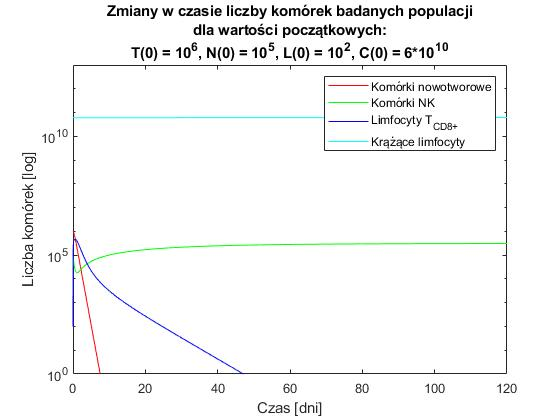
\includegraphics[width=0.85\textwidth]{bez_lecz_sym1_regresja}}
\quad
\subfloat[Zmiany liczby kom�rek badanych populacji dla~warto�ci pocz�tkowej liczby kom�rek nowotworowych $T(0) = 1.8 \cdot 10^{7}$. Stabilizacja liczby kom�rek nowotworowych po~czasie $T_{s}$~$\approx$ 24 dni (576 godzin) oko�o warto�ci $9,8 \cdot 10^{8}$.]{\label{bez_lecz_brak_stlumienia}
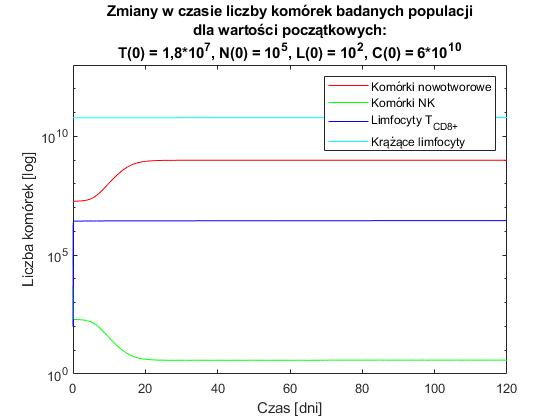
\includegraphics[width=0.85\textwidth]{bez_lecz_sym1_progres}}
\caption{Wykresy zmian liczby kom�rek badanych populacji -- kom�rek nowotworowych $T(t)$, kom�rek NK $N(t)$, limfocyt�w $T_{CD8+}$ $L(t)$ i~limfocyt�w kr���cych $C(t)$.}
\label{zmiany_liczby_kom_4_populacji}
\end{figure}

Na~pierwszym wykresie (Rys. \ref{bez_lecz_stlumienie}) przedstawiono regresj� nowotworu wskutek dzia�ania uk�adu immunologicznego po~oko�o 7 dniach.
Wykres drugi (Rys. \ref{bez_lecz_brak_stlumienia}) obrazuje przypadek, w~kt�rym uk�ad immunologiczny nie jest w~stanie pokona� nowotworu -- liczba jego kom�rek stabilizuje si� po~24 dniach oko�o warto�ci $9,8 \cdot 10^{8}$ (odpowiada to~obj�to�ci 980 $mm^{3}$ i~d�ugo�ci promienia 6,16 $mm$).

\newpage
\indent Zmiany wielko�ci nowotworu otrzymane na~koniec symulacji trwaj�cej $T_{k}$ = 120 dni w~zale�no�ci od~pocz�tkowej liczby kom�rek nowotworowych $T(0)$ przedstawiono na~wykresie (Rys. \ref{wykres_bez_lecz_t120_t0}). 

\begin{figure}[!htb]
	\centering
	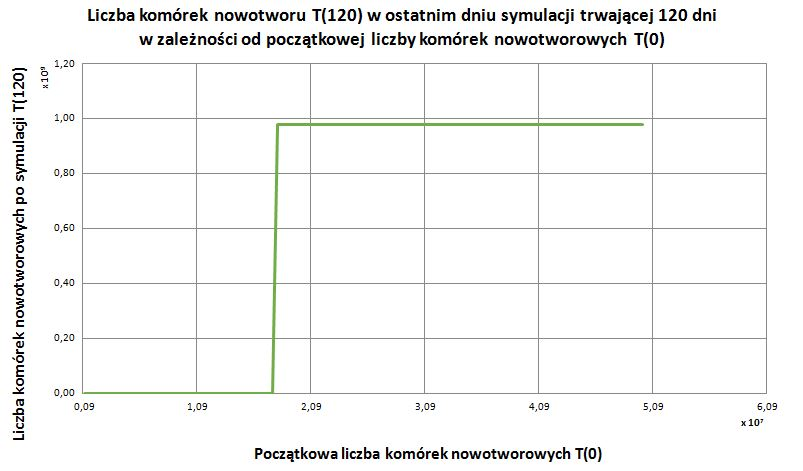
\includegraphics[width=1\textwidth]{wykres_bez_lecz_t120_t0}
	\caption{Wyniki otrzymane na~koniec symulacji, kt�ra trwa�a $T_{k}$ = 120 dni. Liczba kom�rek nowotworowych na~koniec symulacji $T(120)$ w~zale�no�ci od~pocz�tkowej liczby kom�rek nowotworowych $T(0)$.}\label{wykres_bez_lecz_t120_t0} 
\end{figure}

\newpage
Na~wykresie (Rys. \ref{wykres_bez_lecz_promien_t0}) pokazano zmiany d�ugo�ci promienia nowotworu otrzymane na~koniec symulacji trwaj�cej $T_{k}$ = 120 dni w~zale�no�ci od~pocz�tkowej liczby kom�rek nowotworowych $T(0)$.

\begin{figure}[!htb]
	\centering
	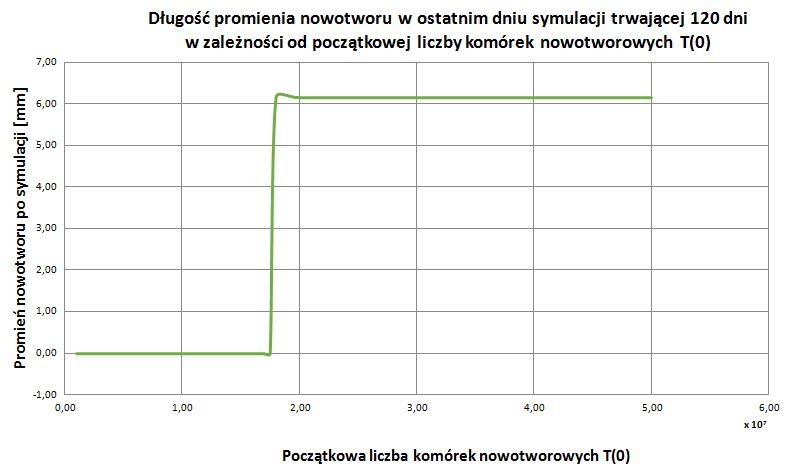
\includegraphics[width=1\textwidth]{wykres_bez_lecz_promien_t0}
	\caption{Wyniki otrzymane na~koniec symulacji, kt�ra trwa�a $T_{k}$ = 120 dni. D�ugo�� promienia nowotworu [mm] na~koniec symulacji w~zale�no�ci od~pocz�tkowej liczby kr���cych limfocyt�w $T(0)$.}\label{wykres_bez_lecz_promien_t0} 
\end{figure}

Wnioski:
\begin{itemize}
\item zdrowy uk�ad immunologiczny jest w~stanie zniszczy� kom�rki nowotworowe przy~wykorzystaniu wy��cznie kom�rek wyst�puj�cych naturalnie w~organizmie (kom�rek NK, limfocyt�w $T_{CD8+}$, limfocyt�w kr���cych) bez ingerencji dodatkowych czynnik�w (np. leczenia);
\item przy~zbyt~du�ej pocz�tkowej liczbie kom�rek nowotworu ($T(0) = 1,8 \cdot 10^{7}$) uk�ad immunologiczny nie jest w~stanie samoistnie pozby� si� nowotworu.
\end{itemize}

\newpage
\subsection{Scenariusz II -- symulacja wykonana dla modelu nieleczonego guza}

\noindent \textbf{Podejmowany problem:} \newline Analiza zmian odpowiedzi uk�adu immunologicznego w~zale�no�ci od~pocz�tkowej liczby limfocyt�w kr���cych $C(0)$ (badanie stanu uk�adu immunologicznego na~podstawie wielko�ci nowotworu po zadanym czasie symulacji).

\noindent \newline \textbf{Warunki pocz�tkowe:} \newline Wielko�� (tj., liczb� kom�rek) nowotworu $T(0)$, liczb� kom�rek NK $N(0)$, liczb� limfocyt�w $T_{CD8+}$ oraz liczb� limfocyt�w kr���cych $C(0)$ dobrano jak~w~tabeli \ref{warunki_poczatkowe_bez}, a~nast�pnie do�wiadczalnie zmieniano warto�� pocz�tkowej liczby limfocyt�w kr���cych $C(0)$.

\noindent \newline \textbf{Przyj�te parametry:} \newline Parametry dla~modelu nieuwzgl�dniaj�cego leczenia jak~w~tabeli \ref{parametry_modelu}.

\noindent \newline \textbf{Czas symulacji:} \newline $T_{k}$ = 120 dni \newline \newline W~tabeli \ref{zmiany_poczatkowej_wartosci_C} przedstawiono pocz�tkow� liczb� limfocyt�w kr���cych $C(0)$, liczb� kom�rek nowotworu po~symulacji w~chwili $T_{k}$ = 120 dni $T(120)$ oraz~szacowan� obj�to�� i~d�ugo�� promienia nowotworu po~symulacji w~chwili $T_{k}$ = 120 dni.

\begin{table}[!htb]
\caption{Pocz�tkowa liczba limfocyt�w kr���cych $C(0)$, liczba kom�rek nowotworowych po~symulacji w~chwili $T_{k}$ = 120 dni $T(120)$ oraz~szacowana obj�to�� i~d�ugo�� promienia nowotworu po~symulacji w~chwili $T_{k}$ = 120 dni.}\label{zmiany_poczatkowej_wartosci_C}
	\centering
\begin{tabular}{|c|c|c|c|} \hline \hline
		$C(0)$ & $T(120)$ & Obj�to�� & Promie� \\
		$[$liczba kom�rek$]$ & $[$liczba kom�rek$]$ & nowotworu [$mm^{3}$] & nowotworu [mm] \\ \hline
		$6 \cdot 10^{10}$ & $6,76 \cdot 10^{-8}$ & $6,76 \cdot 10^{-14}$ & $2,5 \cdot 10^{-5}$ \\ \hline
		$3 \cdot 10^{10}$ & $1,69 \cdot 10^{-7}$ & $1,69 \cdot 10^{-13}$ & $3,4 \cdot 10^{-5}$ \\ \hline
		$1 \cdot 10^{10}$ & $3,09 \cdot 10^{-8}$ & $1,33 \cdot 10^{-14}$ & $1,5 \cdot 10^{-5}$ \\ \hline
		$6 \cdot 10^{9}$ & $4,79 \cdot 10^{-8}$ & $4,79 \cdot 10^{-14}$ & $2,3 \cdot 10^{-5}$ \\ \hline
		$4 \cdot 10^{9}$ & $5,72 \cdot 10^{-8}$ & $5,72 \cdot 10^{-14}$ & $2,4 \cdot 10^{-5}$ \\ \hline
		$3,5 \cdot 10^{9}$ & $9,8 \cdot 10^{8}$ & $980$ & $6,16$ \\ \hline
		$3 \cdot 10^{9}$ & $9,8 \cdot 10^{8}$ & $980$ & $6,16$ \\ \hline
		$1 \cdot 10^{9}$ & $9,8 \cdot 10^{8}$ & $980$ & $6,16$ \\ \hline
		$6 \cdot 10^{8}$ & $9,8 \cdot 10^{8}$ & $980$ & $6,16$ \\ \hline
		$3 \cdot 10^{8}$ & $9,8 \cdot 10^{8}$ & $980$ & $6,16$ \\ \hline
		\end{tabular}
\end{table}

Zmiany liczby kom�rek badanych populacji - kom�rek nowotworowych $T(t)$, kom�rek NK $N(t)$, limfocyt�w $T_{CD8+}$ $L(t)$ i~limfocyt�w kr���cych $C(t)$ przedstawiono na~wykresach (Rys. \ref{zmiany_liczby_kom_4_populacjiC}).

\begin{figure}
\centering
\subfloat[Zmiany liczby kom�rek badanych populacji dla~warto�ci pocz�tkowej liczby limfocyt�w kr���cych $C(0) = 6 \cdot 10^{10}$. Regresja nowotworu po~czasie $T_{r}$~$\approx$ 7 dni (168 godzin).]{\label{bez_lecz_stlumienieC}
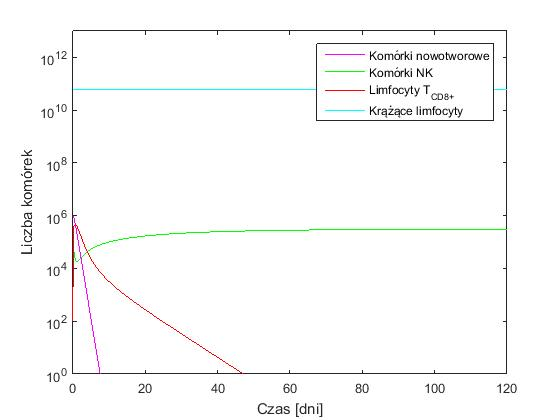
\includegraphics[width=0.85\textwidth]{bez_lecz_sym2_regresja}}
\quad
\subfloat[Zmiany liczby kom�rek badanych populacji dla~warto�ci pocz�tkowej liczby limfocyt�w kr���cych $C(0) = 3,5 \cdot 10^{9}$. Stabilizacja liczby kom�rek nowotworowych po~czasie $T_{s}$~$\approx$ 28 dni (672 godziny) oko�o wartosci $9,8 \cdot 10^{8}$.]{\label{bez_lecz_brak_stlumieniaC}
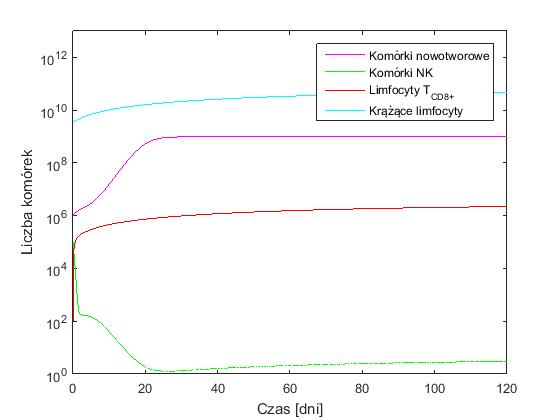
\includegraphics[width=0.85\textwidth]{bez_lecz_sym2_progres}}
\caption{Wykresy zmian liczby kom�rek badanych populacji -- kom�rek nowotworowych $T(t)$, kom�rek NK $N(t)$, limfocyt�w $T_{CD8+}$ $L(t)$ i~limfocyt�w kr���cych $C(t)$.}
\label{zmiany_liczby_kom_4_populacjiC}
\end{figure}

\newpage
Na~pierwszym z~nich (Rys. \ref{bez_lecz_stlumienieC}) przedstawiono regresj� nowotworu wskutek dzia�ania odpowiednio silnego uk�adu immunologicznego po~oko�o 7 dniach. Na~drugim wykresie (Rys. \ref{bez_lecz_brak_stlumieniaC}) liczba kom�rek nowotworowych stabilizuje si� po~28 dniach oko�o warto�ci $9,8 \cdot 10^{8}$ (odpowiada to~obj�to�ci 980 $mm^{3}$ i~d�ugo�ci promienia 6,16 $mm$). Uk�ad immunologiczny ze wzgl�du na~zmniejszon� liczb� kr���cych limfocyt�w jest zbyt s�aby, by zniszczy� kom�rki nowotworu.
\newline \newline \indent Zmiany wielko�ci nowotworu otrzymane na~koniec symulacji trwaj�cej $T_{k}$ = 120 dni w~zale�no�ci od~pocz�tkowej liczby kr���cych limfocyt�w $C(0)$ przedstawiono na~wykresie (Rys. \ref{wykres_bez_lecz_t120_c0}). 

\begin{figure}[!htb]
	\centering
	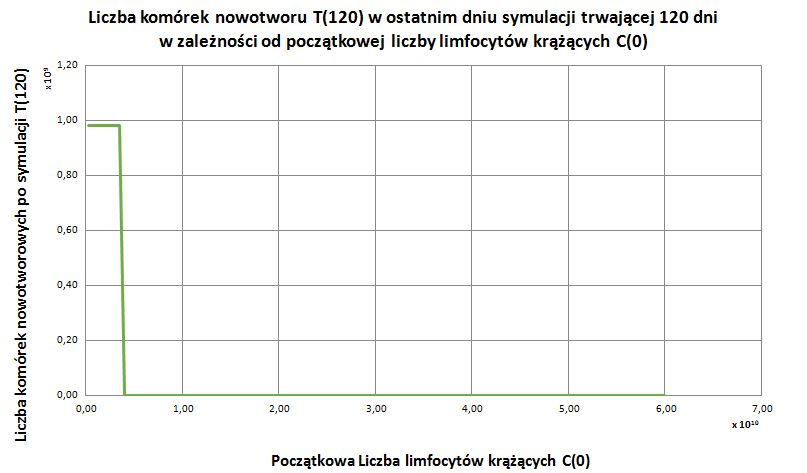
\includegraphics[width=1\textwidth]{wykres_bez_lecz_t120_c0}
	\caption{Wyniki otrzymane na~koniec symulacji, kt�ra trwa�a $T_{k}$ = 120 dni. Liczba kom�rek nowotworowych na~koniec symulacji $T(120)$ w~zale�no�ci od~pocz�tkowej liczby kr���cych limfocyt�w $C(0)$.}\label{wykres_bez_lecz_t120_c0} 
\end{figure}

\newpage
Na~wykresie (Rys. \ref{wykres_bez_lecz_promien_c0}) pokazano zmiany d�ugo�ci promienia nowotworu otrzymane na~koniec symulacji trwaj�cej $T_{k}$ = 120 dni w~zale�no�ci od~pocz�tkowej liczby kr���cych limfocyt�w $C(0)$.

\begin{figure}[!htb]
	\centering
	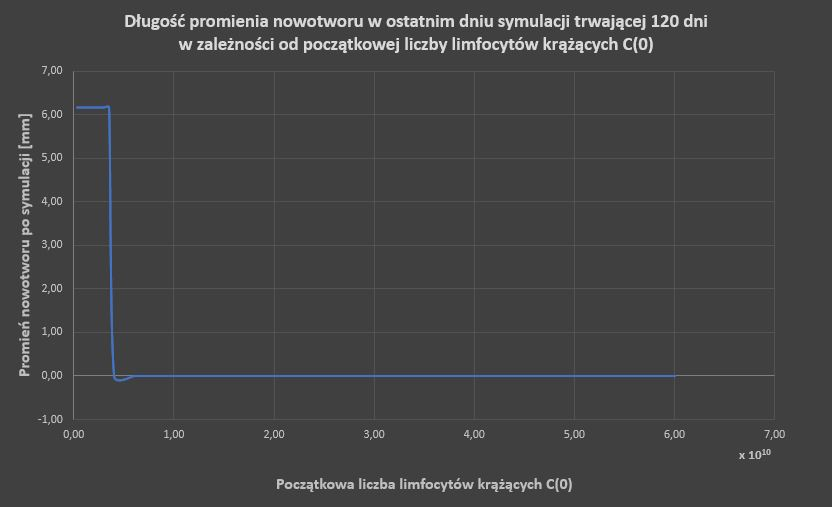
\includegraphics[width=1\textwidth]{wykres_bez_lecz_promien_c0}
	\caption{Wyniki otrzymane na~koniec symulacji, kt�ra trwa�a $T_{k}$ = 120 dni. D�ugo�� promienia nowotworu [mm] na~koniec symulacji w~zale�no�ci od~pocz�tkowej liczby kr���cych limfocyt�w $C(0)$.}\label{wykres_bez_lecz_promien_c0} 
\end{figure}

Wnioski:
\begin{itemize}
\item przy~odpowiednio du�ej liczbie kr���cych limfocyt�w ($C(0) \approx 4 \cdot 10^{9}$) uk�ad immunologiczny jest w~stanie zniszczy� kom�rki nowotworowe bez ingerencji zewn�trznych czynnik�w (np. leczenia),
\item przy~zbyt ma�ej liczbie kr���cych limfocyt�w (z�y stan uk�adu immunologicznego) organizm nie jest w~stanie zniszczy� kom�rek nowotworowych.
\end{itemize} 

\newpage
\section{Leczenie metod� chemioterapii}
\section{Leczenie metod� immunoterapii}
\section{Po��czenie metod chemioterapii i~immunoterapii}

\chapter{Rezultaty}
\chapter{Analiza wynik�w}
\chapter{Podsumowanie}

%nowe
Nowo odkryta odmiana limfocyt�w T...
%nowe

\begin{thebibliography}{9}
\bibitem{1} Mustafa Mamat, Subiyanto i~Agus Kartono, ,,Mathematical Model of Cancer Treatments Using Immunotherapy, Chemotherapy and Biochemotherapy",
\bibitem{2} R. Tadeusiewicz, ,,Biocybernetyka. Metodologiczne podstawy dla in�ynierii biomedycznej.�, PWN, 2013
\bibitem{3} Redaktor naukowy dr n. med. Janusz Meder, ,,Podstawy onkologii klinicznej", Centrum Medyczne Kszta�cenia Podyplomowego w~Warszawie, 2011
\bibitem{4} Ewelina Dymarska, ,,Czynniki moduluj�ce uk�ad immunologiczny cz�owieka", Uniwersytet Ekonomiczny we Wroc�awiu, Zeszyty Naukowe Pa�stwowej Wy�szej Szko�y Zawodowej im. Witelona w~Legnicy nr 19(2)/2016
\bibitem{5} Nadzieja Drela, ,,Immunologiczna teoria starzenia", Wydzia� Biologii Uniwersytetu Warszawskiego, Instytut Zoologii, Zak�ad Immunologii, Warszawa, 23 kwietnia 2014
\bibitem{6} Marta Sochocka, Zofia B�ach-Olszewska, ,,Mechanizmy wrodzonej odporno�ci", Laboratorium Wirusologii Instytutu Immunologii i~Terapii Do�wiadczalnej Polskiej Akademii Nauk im L. Hirszfelda we Wroc�awiu, Post�py Hig Med Do�w., 59: 250-258, 2005
\bibitem{7} Emilia Kolarzyk, ,,Wybrane problemy higieny i~ekologii cz�owieka", Wydawnictwo Uniwersytetu Jagiello�skiego, Krak�w, 2008, wyd.1
\bibitem{8} Beata Tokarz-Deptu�a, Tymoteusz Miller, Wies�aw Deptu�a, ,,Cytokiny z~rodziny interleukiny-1", Katedra Mikrobiologii i~Immunologii, Wydzia� Nauk Przyrodniczych, Uniwersytet Szczeci�ski
\bibitem{9} ,,Chemioterapia, Immunoterapia i~Terapia Celowana Informacje dla Pacjenta", Centrum Onkologii Ziemi Lubelskiej im. �w. Jana z~Dukli, Lublin, 2011
\bibitem{10} Jacek Mackiewicz, Andrzej Mackiewicz, ,,Immunoterapia nowotwor�w i~perspektywy jej rozwoju", Zak�ad Immunologii Nowotwor�w, Katedra Biotechnologii Medycznej, Uniwersytet Medyczny im. Karola Marcinkowskiego w~Poznaniu, Wielkopolskie Centrum Onkologii w~Poznaniu
\bibitem{11} Anna �wieboda-Sadlej, ,,Skojarzone leczenie nowotwor�w � wsp�praca chirurga i~onkologa klinicznego w~zakresie leczenia raka piersi, jelita grubego i~p�uca", Klinika Hematologii, Onkologii i~Chor�b Wewn�trznych WUM
\bibitem{12} Ewa Sikora, ,,Cykl kom�rkowy i~apoptoza: �mier� starej kom�rki'', Polskie Towarzystwo Biochemiczne, ,,Post�py biochemii'', tom 42, nr 2, 1996
\bibitem{13} Izabela Klaska, Jerzy Z. Nowak, ,,Rola uk�adu dope�niacza w~fizjologii i~patologii'', ��d�, 2007
\bibitem{14} dr hab. Krzysztof Bryniarski, ,,Immunologia'', 2017
\bibitem{15} W�odzimierz Ma�li�ski, Ewa Kontny, ,,Podstawy immunologii dla reumatolog�w'', Narodowy Instytut Geriatrii, Reumatologii i~Rehabilitacji, Warszawa, 2015
\bibitem{16} Aleksandra E. Tokarz, Iwona Szu�cik, Agnieszka �y�ka, Ewa St�pie�, ,,Wykorzystanie mikromacierzy w ocenie prozapalnych i proangiogennych cytokin w patomechanizmie retinopatii cukrzycowej'', 2014
\bibitem{17} K. Morka, G. Bugla-P�osko�ska, ''Medycyna do�wiadczalna i mikrobiologia'', 2017
\bibitem{18} O.G. Isaeva and V.A. Osipov, ,,Different strategies for cancer treatment: Mathematical modelling'', 2009
\bibitem{19} L.G. de Pillisa, W. Gu, A.E. Radunskayb, ,,Mixed immunotherapy and chemotherapy of tumors: modeling,
applications and biological interpretations'', 2005
\bibitem{20} Krzysztof Wiktorowicz, Krzysztof Kaszkowiak, ,,Budowa i funkcja ludzkich antygen�w zgodno�ci tkankowej. Cz�� 1. Kodowanie i budowa'', Katedra Biologii i Ochrony �rodowiska, Uniwersytet Medyczny im. Karola Marcinkowskiego w Poznaniu, 2018
\bibitem{21} Dominik Strzelecki, Tomasz Pawe�czyk, Jolanta Rabe-Jab�o�ska, ,,Zaburzenia depresyjne w przebiegu leczenia przewlek�ego wirusowego zapalenia w�troby interferonem $\alpha$", Post�py Psychiatrii i Neurologii, 2005
\bibitem{22} Waldemar Halota, Ma�gorzata Paw�owska, Michai� Andrejczyn, ,,Interferony alfa w leczeniu przewlek�ych zaka�e� HCV", Przegl�d epidemiologiczny, 2004
\bibitem{23} Ugo Del Monte, ,,Does the cell number $10^{9}$ still really fit one gram of tumor tissue?'', Cell Cycle, 8:3, 505-506, 2009
\bibitem{24} Marcus C.B. Tan, Peter S. Goedegebuure, Timothy J. Eberlein, ,,Chirurgia onkologiczna cz�� V'',  Chirurgia Sabistona, rozdzia� 29 ,,Biologia nowotwor�w i markery nowotworowe'', 2012
\bibitem{25} Monika Olsz�wka, Kamil Maci�g, ,,Choroby nowotworowe: wybrane zagadnienia'', Fundacja na rzecz promocji nauki i rozwoju TYGIEL, Lublin, 2015
\bibitem{26} El�bieta Ograczyk, Magdalena Kowalewicz-Kulbat, Sebastian Wawrocki, Marek Fol, ,,Immunosupresja � wymagaj�cy sprzymierzeniec na trudne czasy'', Uniwersytet ��dzki, Katedra Immunologii i Biologii Infekcyjnej, ��d�, 2015
\bibitem{27} Zdzis�aw Gli�ski, Krzysztof Kostro, ,,Immunoonkologia � nowe dane'', �ycie Weterynaryjne 91(11), Wydzia� Medycyny Weterynaryjnej w Lublinie, 2016
\bibitem{28} Lek. med. Marta Adamczyk?Korbel, ,,Uk�ad odporno�ciowy cz�owieka a probiotyki'', Klinika Pneumonologii, Onkologii I Alergologii, Lublin, Medycyna i pasje, Medycyna zapobiegawcza, luty 2010
\bibitem{29} Zuzanna Wyszy�ska, Lidia Szulc, Justyna Struzik, Marek Niemia�towski, ,,Immunobiologia kom�rek NK'', Zak�ad Immunologii Katedry Nauk Przedklinicznych Wydzia�u Medycyny Weterynaryjnej SGGW, Warszawa, 2012
\end{thebibliography}


%\appendix  % <--- zaczynaj� si� dodatki; jak nazywa si� rozdzia� -> szuka� appendixname powy�ej
\chapter{Dodatek}

\section{Tabela skr�t�w}

\begin{table}[!htb]
	\centering
	\topcaption{Skr�ty wykorzystane w pracy}\label{Tabelka_Tabela}
	\begin{tabular}{|c|c|c|c|} \hline \hline 
		Skr�t & Nazwa angielska & Nazwa polska \\ \hline
		TIL & Tumor Infiltrating Lymphocytes & Limfocyty naciekaj�ce nowotw�r \\ \hline
		NK & Natural killers & Naturalni zab�jcy \\ \hline
		IL-2 & Interleukina-2 & Interleukina-2 \\ \hline
		INF-${\alpha}$ & Interferon-${\alpha}$ & Interferon-${\alpha}$ \\ \hline
		MBL & Mannose Binding Lectin & Lektyna wi���ca mannoz� \\ \hline
		APC & Antigen Presenting Cells & Kom�rki prezentuj�ce antygen \\ \hline
		NCRs & Natural Cytotoxicity Receptors & Receptory naturalnej cytotoksyczno�ci \\ \hline
		KIR & Killer cells Inhibitory Receptor & Receptor hamuj�cy zab�jcze kom�rki \\ \hline
		ISRE & Interferon-Stimulated & Element odpowiedzi \\
		& Response Element & stymulowanej przez interferon  \\ \hline
		TCGF & T Cell Growth Factor & Czynnik wzrostu kom�rek T \\ \hline
		FDA & Food and~Drug Administration & Agencja �ywno�ci i~lek�w \\ \hline
		AICD & Activation-Induced Cell Death & �mier� kom�rek indukowana aktywacj� \\ \hline
		TNF$_{\alpha}$ & Tumor Necrosis Factor $\alpha$ & Czynnik martwicy guza $\alpha$ \\ \hline
		CIPN & Chemotherapy-Induced  & Obwodowa polineuropatia \\	
		& Peripheral Neuropathy & wywo�ana chemioterapi� \\ \hline
		LAK & Lymphokine Activated Killers & Kom�rki zab�jcze aktywowane limfokin� \\ \hline
		HSP & Heat Shock Protein & Bia�ka szoku cieplnego \\ \hline
		DC & Dendritic cells & Kom�rki dendrytyczne \\ \hline
		
		
	\end{tabular}
\end{table}

%%%%%%%%%%%%%%%%%%%%%%%%%%%%%%%%%%%%%%%%%%%%%%%%%%%%%%%%%%%%%%%%%%%%%%%%%%%%%%%%%%%%%%%%%%%%%%%%%%%%%%%%%%%%%%%%%%%%%%%%%%%%%%%%%%%%%%%%%%%%%%%%%%%%%%%%%%%%%%%%%%%%%%%
 
%\chapter{Dodatek B}
Podstawowe kwestie techniczne dotycz�ce wzor�w, rysunk�w, tabel poni�ej.

Wzory tworzymy w �rodowisku \texttt{equation}. Chc�c odwo�a� si� do wybranego wzoru gdzie� w tek�cie nale�y nada� mu stosown�, niepowtarzaln� i jednoznaczn� etykiet�, po ty by m�c np. napisa� zdanie: ze wzoru~\ref{Wzor_Dodawanie} wynika \ldots
\begin{equation}\label{Wzor_Dodawanie}
	c = a + b
\end{equation}

Wzory z�o�one, charakteryzuj�ce si� przypisaniem warto�ci zmiennej w pewnych okoliczno�ciach tworzymy przy u�yciu otoczenia \texttt{eqnarray}. Odwo�anie do wzoru jak wcze�niej. 
\begin{eqnarray}\label{equ_progowanie}
    BW & = & \left \{
    \begin{array}{ll}
      1, & I(x,y) \geq T \\
      0, & I(x,y) < T\\
    \end{array}
    \right.,
\end{eqnarray}

% \subsection{Usuwanie numeracji przy r�wnaniach}

Numeracj� r�wna� mo�na tymczasowo (w~danej linijce) wy��czy� poprzez u�ycie $\backslash{}nonumber$
\begin{eqnarray}
	a_i = a_{i-1}+a_{i-2}\nonumber \\ % w tej linijce nie ma numeru
              +a_{i-3}
\end{eqnarray}


\section{Wstawianie rysunk�w}
Rysunki umieszczamy w otoczeniu \texttt{figure}, centruj�c je w poziomie komend� \texttt{centering}. Rozmiary rysunku ustalamy w komendzie \texttt{includegraphics} dobieraj�c wielko�� wzgl�dem rozmiaru strony lub bezwzgl�dnie np. w cm. Ponadto najpierw zapowiadamy pojawienie si� rysunku w tek�cie (czyli np. Na rysunku (Rys~\ref{Rysunek_LogoIB}) pracy, a dopiero p�niej wstawiamy sam rysunek. Dodatkowo sterowa� mo�emy umiejscowieniem rysunku na stronie dzi�ki parametrom \texttt{[!htb]} okre�laj�cym miejsce. Odpowiednio s� to: \texttt{here}, \texttt{top}, \texttt{bottom}. 
\begin{figure}[!htb]
	\centering
	
\includegraphics[width=.35\textwidth]{logoRIB}
	\caption{Logo Wydzia�u In�ynierii Biomedycznej.}\label{Rysunek_LogoIB}
\end{figure}

Do��czaj�c rysunki nie trzeba podawa� rozszerzenia (wr�cz jest to odradzane). Je�li rysunki znajduj� si� w~katalogu \emph{rysunki}, nie trzeba r�wnie� podawa� �cie�ki do nich.

\section{Wstawianie tabelek}
Analogicznie post�pujemy z tabelkami, z t� r�nic� �e tworzymy j� w otoczeniu \texttt{table}. W nim natomiast sam� tabel� definiujemy albo w �rodowisku \texttt{tabular}, albo \texttt{tabularx}. Podobnie z odwo�aniami w tek�cie: najpierw odwo�anie w Tab.~\ref{Tabelka_Tabela}, a dopiero p�niej sama tabela.
\begin{table}[!htb]
	\centering
	\topcaption{Opis nad tabelk�.}\label{Tabelka_Tabela}
	\begin{tabular}{|c|c|c|c|} \hline \hline 
		Kolumna 1 & Kolumna 2 & Kolumna 3 & Kolumna 4 \\ \hline
		Wiersz 1 & & & \\ \hline
		Wiersz 2 & & & \\ \hline
		Wiersz 3 & & & \\ \hline
		& & & \\ \hline
		& & & \\ \hline
	\end{tabular}
\end{table}

%%%%%%%%%%%%%%%%%%%%%%%%%%%%%%%%%%%%%%%%%%%%%%%%%%%%%%%%%%%%%%%%%%%%%%%%%%%%%%%%%%%%%%%%%%%%%%%%%%%%%%%%%%%%%%%%%%%%%%%%%%%%%%%%%%%%%%%%%%%%%%%%%%%%%%%%%%%%%%%%%%%%%%%
\chapter{Kwestie edytorskie}
Zbi�r zasad pomocnych przy redagowaniu tekstu pracy wystarczaj�co szczeg�owo przedstawia ksi��ka~\cite{Chwalowski}.

Uwaga! Pisz�c prac� nale�y zwr�ci� uwag� na nast�puj�ce kwestie:
\begin{enumerate}
	\item Prace piszemy w formie bezosobowej.
	\item Unikamy okre�le� potocznych, spolszcze� funkcjonuj�cych codziennej mowie itp.
	\item Pos�uguj�c si� znanymi nam (a nie czytelnikowi) has�ami (r�wnie� skr�tami, akronimami) najpierw je definiujemy i~t�umaczymy, a~dopiero p�niej traktujemy za znane.
	\item Podpisy pod rysunkami lub nad tabelami traktujemy jak zdania, a wi�c powinny stanowi� sp�jn� ca�o�� oraz powinny zosta� zako�czone kropk�.
	\item Podobnie wypunktowania (po dwukropku kolejne punkty pisane ma�ymi literami, oddzielane przecinkami, ostatni zako�czony kropk� o ile ko�czy zdanie).
	\item Do ka�dego rysunku, tabeli, pozycji bibliograficznej musi istnie� odwo�anie w tek�cie pracy, przy czym do pierwszych dw�ch musi si� ono pojawi� zanim umie�cimy rysunek/tabel�.
\end{enumerate}


\clearpage \addcontentsline{toc}{chapter}{\bibname}
%\bibliography{Praca}


\end{document}
